\documentclass[11pt,letterpaper]{article}

\usepackage[T1]{fontenc}
\usepackage[utf8]{inputenc}
\usepackage{lmodern}
\usepackage{microtype}
\usepackage[margin=1.1in]{geometry}
\usepackage{amsmath,amssymb,bm}
\usepackage{siunitx}      % for \si{\angstrom}
\usepackage{physics}      % for \dyad{}{}
\ExplSyntaxOn
\msg_redirect_name:nnn { siunitx } { physics-pkg } { none }
\ExplSyntaxOff
\AtBeginDocument{\RenewCommandCopy\qty\SI}
\usepackage{graphicx}
\graphicspath{{figures/}{../figures/}{./}}
\usepackage{subcaption}
\usepackage{booktabs,tabularx}
\usepackage[section]{placeins}
\usepackage{needspace}
\usepackage[font=small,labelfont=bf,labelsep=period,
  justification=justified,singlelinecheck=false]{caption}
\captionsetup[figure]{position=bottom,skip=6pt}
\captionsetup[table]{position=top,skip=6pt}
\renewcommand{\arraystretch}{1.15}
\usepackage{titlesec}
\usepackage[numbers,sort&compress]{natbib}
\setcitestyle{super,comma,numbers,sort&compress}
\usepackage[dvipsnames]{xcolor}
\usepackage[hidelinks]{hyperref}

% Keep paragraph headings at their semantic level, but display them as
% unnumbered block headings rather than run-in headings.
\setcounter{secnumdepth}{3}
\titleformat{\paragraph}[block]
  {\normalfont\normalsize\bfseries}
  {}
  {0pt}
  {}
\titlespacing*{\paragraph}
  {0pt}
  {1.4\baselineskip}
  {0.35\baselineskip}

% Supporting-information numbering for sections, figures, and equations.
\renewcommand{\thesection}{S\arabic{section}}
\renewcommand{\thesubsection}{\thesection.\arabic{subsection}}
\renewcommand{\theequation}{S\arabic{equation}}
\renewcommand{\thefigure}{S\arabic{figure}}
\renewcommand{\thetable}{S\arabic{table}}
\renewcommand{\thepage}{S\arabic{page}}

\title{Supporting Information for:\\
Two-dimensional powder diffraction in layered van der Waals films:\\
quantitative X-ray area-detector modeling}
\author{}
\date{}


% Explicit placeholders never load scientific results automatically.
\newcommand{\siplaceholder}[2]{%
  \fbox{\begin{minipage}[c][0.14\textheight][c]{\dimexpr\linewidth-2\fboxsep-2\fboxrule\relax}
  \centering\small\textbf{Figure placeholder}\\[0.5em]
  \textbf{#1}\\[0.6em]#2
  \end{minipage}}%
}
\setcounter{tocdepth}{1}

\begin{document}
\maketitle
This Supporting Information follows the physical and experimental sequence of the main manuscript. Sections S1--S5 develop the diffraction model and its detector observable. Section S6 covers the ordered-film comparisons, followed by the PbI$_2$ extension in S7 and calibration, refinement, and uncertainty in S8.
\tableofcontents
\clearpage
\section{Incident beam and scattering geometry}
\label{sec:si_geometric_ray_acceptance}

This section supports the main-text scattering geometry. An incident ray first reaches the sample, and an accepted scattered ray then reaches the active detector. The coordinate definitions below keep those two restrictions separate.

The notation follows the main manuscript. Bold symbols denote vectors or explicitly identified matrices; a hat on a vector denotes unit magnitude, and $\mathsf T$ denotes transpose. The imaginary unit is $i$, and a superscript $*$ denotes complex conjugation except on the reciprocal basis vectors $\mathbf a^*,\mathbf b^*,\mathbf c^*$. Descriptive subscripts such as $\mathrm{det}$, $\mathrm{vol}$ and $\mathrm{proj}$ identify a quantity or coordinate convention. The superscripts $E$, $\mathrm{pre}$, $\mathrm{ROI}$, $\mathrm{meas}$ and $\mathrm{calc}$ label an Ewald-selected quantity, a pre-selection quantity, a region-of-interest average, a measurement and a calculation, respectively. These superscripts identify the role of each quantity.

The laboratory axes are $y$ along the nominal incident beam, $z$ vertical and $x$ transverse. The reciprocal basis vectors include $2\pi$; for the hexagonal setting used here, the basal lattice constant is $a$, the normal repeat is $c$, and $|\mathbf c^*|=2\pi/c$. The source-state index is $s$ throughout. The index $j$ follows the main text: it labels an Ewald-intersection branch in Sec.~\ref{sec:si_detector_profiles} and a parent-rich population in Sec.~\ref{sec:si_pbi2_transition}. Parentheses in $S_{hk}^{(j)}$ identify that population. Subscripts are suppressed only where a fixed rod, source state or population is stated explicitly.


\begin{table}[!htbp]
\centering\small
\caption{Coordinates used in the main text and Supporting Information. Reciprocal basis vectors include $2\pi$.}
\label{tab:si_coordinates}
\begin{tabularx}{\linewidth}{@{}p{0.22\linewidth}X@{}}
\toprule
Symbol & Meaning \\
\midrule
$(h,k,\ell)$ & Integer Miller indices; Bragg orders along a rod occur at $L=\ell$. \\
$L$ & Intrinsic dimensionless coordinate along a crystallite-frame reciprocal rod. \\
$q_z=|\mathbf c^*|L$ & Crystallite-frame film-normal momentum component, as in the main-text stacking model. \\
$Q_z$, $L_{\mathrm{proj}}$ & Projection along the mean film normal, with $L_{\mathrm{proj}}=Q_z/|\mathbf c^*|$. \\
$Q_R$, $r$ & In-plane momentum magnitude and discrete radial-family label $r=h^2+hk+k^2$. \\
$\alpha$, $\beta$ & Crystallite tilt magnitude and azimuth in the two-angle orientation map. \\
$2\theta$, $\phi_f$ & Scattering angle and outgoing-ray azimuth in the declared detector display frame. \\
$x',z'$; $x_D,y_D$ & Main-text in-plane detector axes and SI column/row axes, with $x_D=x'$ and $y_D=-z'$ in the reference pose. \\
\bottomrule
\end{tabularx}
\end{table}
\subsection{Source state and sample intersection}

An incident state $s$ supplies a ray origin $\mathbf r_{0,s}$ and an external incident vector
\begin{equation}
  \mathbf k_{i,s}=\mathbf k_i\!\left(|\mathbf k_{i,s}|,\theta_{i,s},\phi_{i,s}\right),
  \qquad |\mathbf k_{i,s}|=\frac{2\pi}{\lambda_s}.
  \label{eq:si_source_state_vector}
\end{equation}
Here $\lambda_s$ is the source wavelength, $\theta_{i,s}$ is the grazing incidence angle and $\phi_{i,s}$ is the incident azimuth in the declared laboratory frame. The subscripts $i$ and $f$ denote incident and exit quantities. The source-position and angular variables are sampled from the measured Gaussian beam distributions, while $\lambda_s$ is sampled from the specified wavelength spectrum. Writing $\hat{\mathbf s}_{i,s}=\mathbf k_{i,s}/|\mathbf k_{i,s}|$, the incident line, parameterized by path length $\tau$, is
\begin{equation}
\mathbf r_s(\tau)=\mathbf r_{0,s}+\tau\hat{\mathbf s}_{i,s},
\qquad \tau\geq0.
\label{eq:si_incident_ray}
\end{equation}
For the following single-ray geometry equations, the source-state subscript $s$ is suppressed.
Let the sample entrance plane pass through $\mathbf r_{\mathrm S}$ and have outward unit normal $\hat{\mathbf n}$. Solving $(\mathbf r-\mathbf r_{\mathrm S})\cdot\hat{\mathbf n}=0$ gives
\begin{equation}
\tau_{\mathrm{hit}}
=\frac{(\mathbf r_{\mathrm S}-\mathbf r_0)\cdot\hat{\mathbf n}}
       {\hat{\mathbf s}_i\cdot\hat{\mathbf n}},
\qquad
\mathbf r_{\mathrm{hit}}
=\mathbf r_0+\tau_{\mathrm{hit}}\hat{\mathbf s}_i.
\label{eq:si_sample_plane_intersection}
\end{equation}
The sample-intersection test rejects parallel rays and solutions with $\tau_{\mathrm{hit}}\leq0$. For orthonormal in-plane sample directions $\hat{\mathbf e}_1$ and $\hat{\mathbf e}_2$, define
\begin{equation}
\xi_1=(\mathbf r_{\mathrm{hit}}-\mathbf r_{\mathrm S})\cdot\hat{\mathbf e}_1,
\qquad
\xi_2=(\mathbf r_{\mathrm{hit}}-\mathbf r_{\mathrm S})\cdot\hat{\mathbf e}_2.
\label{eq:si_sample_coordinates}
\end{equation}
A rectangular support with width $W$ along $\hat{\mathbf e}_1$ and height $H$ along $\hat{\mathbf e}_2$ accepts the state only if
\begin{equation}
|\xi_1|\leq \frac{W}{2},
\qquad
|\xi_2|\leq \frac{H}{2}.
\label{eq:si_sample_bounds}
\end{equation}
The illuminated footprint is the weighted distribution of the accepted $(\xi_1,\xi_2)$ values. The source distribution and intersection test determine the footprint directly. For the convention in which $\hat{\mathbf n}$ points out of the film, the state-specific grazing angle is
\begin{equation}
\theta_{i,s}
=\sin^{-1}\!\left(-\hat{\mathbf s}_i\cdot\hat{\mathbf n}\right).
\label{eq:si_local_incidence_angle}
\end{equation}
The ordered-film configurations used for the displayed Bi$_2$Se$_3$ and Bi$_2$Te$_3$ calculations specify an unbounded in-plane sample plane. Equation~\eqref{eq:si_sample_bounds} documents the available finite-support model. The retained unbounded-plane geometry excludes sample-edge clipping from the fitted broadening mechanisms.

\subsection{Detector frame and accepted rays}

The detector mapping is most transparent in its own rigid coordinate frame. Its $x_D$ and $y_D$ coordinates increase with detector column and row, respectively, and its plane is $z_D=0$. In the untilted main-text geometry, $x_D$ follows $+x'$ and $y_D$ follows $-z'$, so $+z_D$ is opposite the outward normal $\hat{\mathbf n}_{\mathrm{det}}$. Thus, the main-text $z'$ axis lies in the detector plane, whereas the SI $z_D$ axis is normal to it. Let $\mathbf R_D$ and $\mathbf t_D$ map detector-frame vectors and points into the laboratory frame. For an exit ray that begins at $\mathbf r_{\mathrm{hit}}$ and has unit laboratory direction $\hat{\mathbf s}_f$, the detector-frame origin and direction are
\begin{equation}
\mathbf o_D=\mathbf R_D^{\mathsf T}(\mathbf r_{\mathrm{hit}}-\mathbf t_D),
\qquad
\mathbf s_D=\mathbf R_D^{\mathsf T}\hat{\mathbf s}_f.
\label{eq:si_detector_frame_ray}
\end{equation}
The detector plane is $z_D=0$. Its forward intersection is
\begin{equation}
v_D=-\frac{o_{D,z}}{s_{D,z}},
\qquad
\mathbf p_D=\mathbf o_D+v_D\mathbf s_D,
\label{eq:si_detector_plane_intersection}
\end{equation}
provided $s_{D,z}$ is nonzero and $v_D>0$. The front-face convention additionally requires the exit direction to approach the active face. If $(x_0,y_0)$ is the calibrated reference coordinate and $p_c,p_r$ are the column and row pitches, the dimensionless column and row coordinates are
\begin{equation}
c_D=x_0+\frac{p_{D,x}}{p_c},
\qquad
r_D=y_0+\frac{p_{D,y}}{p_r}.
\label{eq:si_detector_pixel_coordinates}
\end{equation}
For a detector with $N_c$ columns and $N_r$ rows, the active-area condition is
\begin{equation}
-\frac12\leq c_D\leq N_c-\frac12,
\qquad
-\frac12\leq r_D\leq N_r-\frac12.
\label{eq:si_detector_active_bounds}
\end{equation}
The subscripts in $(c_D,r_D)$ distinguish detector coordinates from the lattice repeat $c$ and radial-family label $r$. The beam-center pair $(x_0,y_0)$ follows the main-text calibration convention, in pixel units. The nominal sample-to-detector distance $D$, detector tilts $(\beta_D,\gamma_D)$, and beam center are contained in $\mathbf R_D$, $\mathbf t_D$, and the reference coordinate. Here $D$ denotes the separation along the nominal beam axis in the untilted reference pose. A tilted detector is treated through the full rigid transform. Native pixel masses or finite angular-bin quantities are obtained by integrating the continuous detector-coordinate density over the corresponding region. The coordinate Jacobian that defines the density includes the detector solid-angle factor exactly once.

\subsection{Angular display convention}

For the angular display, $2\theta$ is measured from the declared incident reference direction. The outgoing-ray azimuth $\phi_f$ is measured in the plane perpendicular to that direction, from the upward reference toward the negative column direction. In the untilted laboratory geometry this is from $+z$ toward $-x$. Equivalently, for components in that geometry, $\phi_f=\operatorname{atan2}(-s_{f,x},s_{f,z})$, wrapped to $[-\pi,\pi)$. The same fixed nominal reference is used to remap measured and calculated detector images. This display coordinate is distinct from the incident azimuth $\phi_i$ and crystallite azimuth $\beta$.

\subsection{Source sampling and wavelength dependence}
\label{sec:si_bandwidth_mosaic_scaling}

The source representation samples two transverse positions, two propagation angles, and wavelength. Seeded equal-mass antithetic Latin-hypercube states carry weights $w_s=1/N_s$, where $N_s$ is the source-state count. The position and angular distributions specify the incident beam, whereas the continuous mosaic distribution specifies crystallite orientation. They enter different parts of the calculation. Numerical convergence is discussed in Sec.~\ref{sec:si_workflow}.

For source-state wavelength $\lambda_s$ and incident direction
$\hat{\mathbf s}_{i,s}$, define
\begin{equation}
  k_s=\frac{2\pi}{\lambda_s},
  \qquad
  \mathbf k_{i,s}=k_s\hat{\mathbf s}_{i,s}.
  \label{eq:si_wavelength_sample}
\end{equation}
In reciprocal-space coordinates centered on the origin, the corresponding
Ewald sphere is centered at $-\mathbf k_{i,s}$ and has radius $k_s$.
The integer Bragg vector is $\mathbf G_{hk\ell}=h\mathbf a^*+k\mathbf b^*+\ell\mathbf c^*$. An allowed reciprocal vector contributes only when
\begin{equation}
  \left|\mathbf k_{i,s}+\mathbf G_{hk\ell}\right|=k_s
  \label{eq:si_moving_ewald_condition}
\end{equation}
within the declared instrumental and numerical resolution.\cite{AlsNielsenMcMorrow2001}
The incident direction is resampled as well when beam divergence is included.
Changing wavelength therefore moves the Ewald-sphere center and changes its
radius. The calculation reconstructs and tests Eq.~\eqref{eq:si_moving_ewald_condition}
for every wavelength and direction state. Each wavelength therefore requires its own sphere center as well as its own radius.

For one lattice-plane spacing $d$ at fixed orientation and Bragg angle $\theta_B$, Bragg's law gives a useful
limiting check,
\begin{equation}
  2d\sin\theta_B=\lambda,
  \qquad
  d\theta_B=\frac{d\lambda}{\lambda}\tan\theta_B.
  \label{eq:si_bragg_bandwidth_check}
\end{equation}
This scalar derivative provides a local check on the radial direction in which wavelength changes the detector position. The full detector-space condition retains the coupling among sample orientation, incident direction, mosaicity, refraction, and detector acceptance.

\section{Structural intensity along reciprocal rods}
\label{sec:si_structure_factor_conventions}

The main-text structure factor defines the scattering amplitude of an atomic motif. Finite coherence along the stacking direction converts that amplitude into continuous intensity along a rod. Random in-plane orientation then distributes the rod intensity around a cylinder.

\subsection{Atomic amplitudes and finite stacking}

For in-plane indices $(h,k)$, the unrotated rod is
\begin{equation}
\mathbf G_{hk}(L)=h\mathbf a^*+k\mathbf b^*+L\mathbf c^*.
\label{eq:si_reference_rod}
\end{equation}
The atomic motif amplitude has the phase convention $\exp(i\mathbf G\cdot\mathbf r_a)$, where $\mathbf G$ is the reciprocal vector and $\mathbf r_a$ is the Cartesian position of site $a$. Atomic form factors include their wavelength-dependent anomalous terms. For a sequence of $N$ layers with motif amplitudes $F_{hk,n}$ and reference-position translations $\mathbf t_n$, the coherent amplitude is
\begin{equation}
A_{N,hk}(L,\lambda_s)=\sum_{n=0}^{N-1}F_{hk,n}(L,\lambda_s)
\exp[i\mathbf G_{hk}(L)\cdot\mathbf t_n].
\label{eq:si_finite_stack_amplitude}
\end{equation}
Here $n$ labels layers from $0$ to $N-1$, and $\mathbf t_n$ locates their motif origins in the reference crystallite frame. For fixed $(h,k,L,\lambda_s)$, write $A_N=A_{N,hk}(L,\lambda_s)$. The total finite-stack strength is proportional to $|A_N|^2$. An ensemble of stacking sequences instead gives $\langle|A_N|^2\rangle$, where angle brackets denote the ensemble average. The total-stack and per-layer conventions differ by $N$ and must remain consistent with the population and intensity scale. Section~\ref{sec:si_pbi2_transition} uses an explicitly stated per-trilayer convention.

For identical motifs of amplitude $F$ at one registry, separated by $d$ along the stacking direction, Eq.~\eqref{eq:si_finite_stack_amplitude} reduces to
\begin{equation}
|A_N|^2=|F|^2\left|\sum_{n=0}^{N-1}e^{inq_zd}\right|^2
=|F|^2\frac{\sin^2(Nq_zd/2)}{\sin^2(q_zd/2)},
\qquad q_z=|\mathbf c^*|L.
\label{eq:si_same_registry_laue}
\end{equation}
The removable limit at $q_zd=2\pi m$, for integer $m$, is $N^2|F|^2$. This same-registry example explains finite-width peaks and fringes. A material-specific ordered stack also includes the basal translations of its crystallographic repeat. The native R-centered off-axis Bi$_2$Se$_3$ sequence requires the spacing $d=c/3$ together with its basal translations and crystallographic centering phases in Eq.~\eqref{eq:si_finite_stack_amplitude}.

\subsection{Displacement conventions}

The main text uses Cartesian atomic positions in the phase factor. At an integer Bragg order, the same structure factor can be written in fractional coordinates as
\begin{equation}
F_{hk\ell}(\lambda_s)=\sum_a o_a f_a(Q,\lambda_s)T_a(hk\ell)
\exp\!\left[2\pi i(hx_a+ky_a+\ell z_a)\right].
\label{eq:si_structure_factor_conventional}
\end{equation}
Here $a$ labels atomic sites, $o_a$ is site occupancy, $f_a$ is the atomic scattering factor including anomalous terms, and $(x_a,y_a,z_a)$ are fractional site coordinates. The magnitude is $Q=|\mathbf G_{hk\ell}|$, and $F_{hk\ell}(\lambda_s)=F_{hk}(\ell,\lambda_s)$ uses the main-text rod amplitude at an integer Bragg order. The displacement factor $T_a(hk\ell)$ must be interpreted in the crystallographic convention of the reported $U$ or $B$ parameters. For an isotropic mean-square displacement $U_{\mathrm{iso},a}$,
\begin{equation}
T_a(hk\ell)
=\exp\!\left[-8\pi^2U_{\mathrm{iso},a}
\left(\frac{\sin\theta}{\lambda_s}\right)^2\right]
=\exp\!\left(-\frac12U_{\mathrm{iso},a}Q^2\right),
\label{eq:si_isotropic_displacement_factor}
\end{equation}
with $B_{\mathrm{iso},a}=8\pi^2U_{\mathrm{iso},a}$ and $Q=4\pi\sin\theta/\lambda_s$. Here $\theta$ is half the scattering angle.

The executable CIF interface accepts isotropic $U_{\mathrm{iso}}$ or $B_{\mathrm{iso}}$ values and stores their equivalent isotropic mean-square displacement. The current CIF import is restricted to isotropic displacement metadata. When directional damping is released in the ordered-film parameterization, one shared uniaxial tensor is defined in the film frame,
\begin{equation}
\mathbf U_{\mathrm{film}}
=U_R\left(\mathbf I-\hat{\mathbf n}\hat{\mathbf n}^{\mathsf T}\right)
+U_z\hat{\mathbf n}\hat{\mathbf n}^{\mathsf T},
\label{eq:si_shared_uniaxial_u}
\end{equation}
Here $\mathbf I$ is the three-dimensional identity matrix, and $U_R$ and $U_z$ are the mean-square displacements within the film plane and along its normal $\hat{\mathbf n}$. The resulting directional displacement factor is
\begin{equation}
T_{\mathrm{dir}}(\mathbf Q)
=\exp\!\left[-\frac12\left(U_RQ_R^2+U_zQ_z^2\right)\right].
\label{eq:si_shared_uniaxial_factor}
\end{equation}
This pair describes a shared directional displacement model for the selected ordered structure. A general site-resolved $U_{ij}$ model would additionally require the CIF tensor convention and its transformation into the calculation basis.

\subsection{Rod coverage and radial families}

Reflection identities are constructed before source integration. If $Q_{\max}$ is the largest momentum transfer subtended by the active detector over the wavelength interval and $\Delta Q$ is a declared coverage margin, the symbolic candidate set is
\begin{equation}
\mathcal R=
\left\{(h,k,\ell)\in\mathbb Z^3:
\operatorname{allowed}(h,k,\ell),\;
|\mathbf G_{hk\ell}|\leq Q_{\max}+\Delta Q
\right\}.
\label{eq:si_reflection_candidate_set}
\end{equation}
Here $\operatorname{allowed}$ imposes the reflection conditions of the structural model. For the rod representation, integer $(h,k)$ identities are enumerated by the same detector-coverage rule and the coordinate along each rod remains continuous.

In vacuum, an orientation-independent necessary reach condition is $Q_{R,hk}\leq2k_s$, with $k_s=2\pi/\lambda_s$. The shortest sampled wavelength gives the largest such bound. This bound supplies candidates, while the orientation distribution, optical propagation and active detector impose further restrictions. For a hexagonal basal plane, $Q_R=4\pi\sqrt{r}/(\sqrt{3}a)$ with $r=h^2+hk+k^2$. Each allowed $(h,k)$ member is evaluated individually. The explicit sum accounts for crystallographic multiplicity.

\subsection{Rod measure and powder-cylinder normalization}
\label{subsec:si_rod_measure}

The main text uses a structural density $S_{hk}(L,\lambda_s)$ per unit $L$. Let $S_{q,hk}$ denote the corresponding density per dimensional crystallite-frame coordinate $q_z$. Conservation of intensity requires
\begin{equation}
q_z=|\mathbf c^*|L,\qquad
S_{hk}(L,\lambda_s)\,dL=S_{q,hk}(q_z,\lambda_s)\,dq_z,\qquad
S_{hk}=|\mathbf c^*|S_{q,hk}.
\label{eq:si_rod_measure_conversion}
\end{equation}
Let $P_{hk}$ denote an optional relative population weight of an individual rod. It is separate from the structural density $S_{hk}$ and is included in the combined weight $W_{hk,j,s}$ when the detector density is formed in Sec.~\ref{sec:si_detector_profiles}, following the main-text convention. Uniform azimuth assigns the fraction $d\beta/(2\pi)$ to each azimuth interval. For $Q_R>0$, the physical cylinder area and its intensity density are
\begin{equation}
dA_{\mathrm{cyl}}=Q_R|\mathbf c^*|\,d\beta\,dL,\qquad
\rho_{\mathrm{cyl},hk}=\frac{P_{hk}S_{hk}}{2\pi Q_R|\mathbf c^*|}
=\frac{P_{hk}S_{q,hk}}{2\pi Q_R}.
\label{eq:si_cylinder_density}
\end{equation}
Integration around the circumference recovers the original rod strength. The axial rod has $Q_R=0$ and requires the separate axial treatment because its cylinder circumference vanishes. The full orientation-map determinant in Sec.~\ref{subsec:si_ewald_surface_chart} already contains the azimuthal metric factor.

\section{Mosaic orientation and axial scattering}
\label{sec:si_mosaic}

Crystallite tilt changes which parts of a reciprocal rod meet the elastic condition. This section defines the angular probability used for that weighting, then separates transverse orientation sensitivity from the radial axial extension discussed in the main text.

\subsection{Wrapped mosaic distribution}
\label{subsec:si_wrapped_mosaic}

The wrapped mosaic profile uses a signed tilt coordinate $\Delta\theta\in(-\pi,\pi]$ relative to the substrate normal. Its periodic continuation identifies angles differing by $2\pi$. The component normalization below is with respect to $d\Delta\theta$. The nonnegative tilt magnitude and the density per solid angle use different measures, as specified below.

The profile is a wrapped Gaussian $G_{\mathrm w}$ plus a wrapped Lorentzian $L_{\mathrm w}$. Their mixture weight is $p_{\mathrm{tail}}$, the Lorentzian half-width is $\Gamma$, and the Gaussian standard deviation is $\sigma$:
\[
  \omega_{\mathrm w}(\Delta\theta;p_{\mathrm{tail}},\Gamma,\sigma)
  =p_{\mathrm{tail}}\,L_{\mathrm w}(\Delta\theta;\Gamma)
  +(1-p_{\mathrm{tail}})\,G_{\mathrm w}(\Delta\theta;\sigma),
  \qquad 0\le p_{\mathrm{tail}} \le 1.
\]
The Lorentzian half-width $\Gamma$ and Gaussian standard deviation $\sigma$ are independent. The wrapped Lorentzian and wrapped Gaussian are
\[
  L_{\mathrm w}(\Delta\theta;\Gamma)=
  \sum_{q=-\infty}^{\infty}\frac{1}{\pi}\frac{\Gamma}{(\Delta\theta+2\pi q)^2+\Gamma^2}
  =\frac{1}{2\pi}\,\frac{\sinh\Gamma}{\cosh\Gamma-\cos\Delta\theta},
\]
\[
  \begin{aligned}
    G_{\mathrm w}(\Delta\theta;\sigma)
    &= \sum_{q=-\infty}^{\infty}\frac{1}{\sqrt{2\pi}\sigma}
       \exp\!\left[-\frac{(\Delta\theta+2\pi q)^2}{2\sigma^2}\right] \\
    &= \frac{1}{2\pi}\!\left[
         1+2\sum_{n=1}^{\infty}e^{-n^2\sigma^2/2}\cos(n\Delta\theta)
       \right].
  \end{aligned}
\]
The integer $q$ labels periodic images and $n$ labels positive Fourier harmonics. Angles in these expressions are in radians. Both components integrate to unity over $(-\pi,\pi]$, so $\omega_{\mathrm w}$ is normalized. The underlying unwrapped Lorentzian FWHM is $2\Gamma$, and the underlying unwrapped Gaussian FWHM is $2\sqrt{2\ln 2}\,\sigma$. The local small-width limit recovers the usual line-shape widths, but the refinement and normalization are defined by the wrapped functions above. The broad functional form is phenomenological. These equations define the two-component model. Establishing its necessity requires comparison with a re-optimized Gaussian-only model.

\subsection{Folded tilt probability and orientation measure}

For the even signed profile above, the probability density of the magnitude $0\leq\alpha\leq\pi$ is
\begin{equation}
p_\alpha(\alpha)=\omega_{\mathrm w}(\alpha)+\omega_{\mathrm w}(-\alpha)
=2\omega_{\mathrm w}(\alpha),\qquad
p_m(\alpha,\beta)=\frac{p_\alpha(\alpha)}{2\pi}.
\label{eq:si_folded_orientation}
\end{equation}
Thus $\int_0^\pi p_\alpha\,d\alpha=1$ and $\int_0^\pi\int_0^{2\pi}p_m\,d\beta\,d\alpha=1$. The angular-line measure uses the flat coordinate element $d\alpha\,d\beta$. When the same normal directions are expressed as a density per solid angle, $d\Omega=\sin\alpha\,d\alpha\,d\beta$, the corresponding density is
\begin{equation}
f_\Omega(\alpha,\beta)=\frac{p_\alpha(\alpha)}{2\pi\sin\alpha},
\qquad 0<\alpha<\pi.
\label{eq:si_orientation_solid_angle}
\end{equation}
The apparent polar singularity is integrable with the solid-angle measure. On a sphere of radius $Q$, the density per surface area is $f_\Omega/Q^2$. A smooth density specified directly per solid angle is a different orientation law. Figure~\ref{fig:si_mosaic_measures} shows these probability conventions.

\begin{figure}[!htbp]
\centering
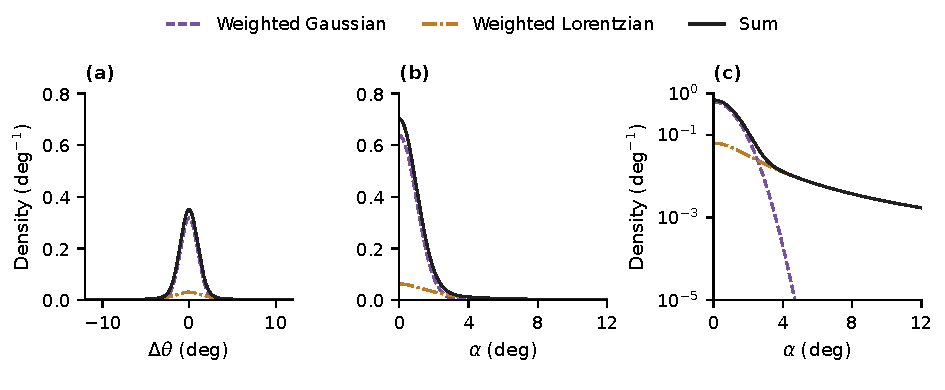
\includegraphics[width=\linewidth]{figures/mosaic_measure_guide.pdf}
\caption{Wrapped angular distributions and their measures. Purple dashed and amber dash-dotted lines show the weighted Gaussian and Lorentzian components, and the black solid line is their sum. (a) Signed density versus $\Delta\theta$. (b) The folded magnitude density on the same linear ordinate scale. (c) The same folded curves on a logarithmic ordinate scale. The parameter values are $\sigma=1^\circ$, $\Gamma=2^\circ$, and $p_{\mathrm{tail}}=0.2$, with azimuth uniform. Ordinates are probability density per degree. Each component is normalized over the complete angular domain before applying its mixture weight, and the displayed windows retain that full-domain normalization. Folding adds the positive and negative signed contributions. The wider component remains visible away from the core.}
\label{fig:si_mosaic_measures}
\end{figure}

The orientation map rotates the entire reciprocal rod, including its basal offset. For the positive-$L$ axial rod, the geometry simplifies to
\begin{equation}
Q_R=|\mathbf c^*|L\sin\alpha,\qquad Q_z=|\mathbf c^*|L\cos\alpha.
\label{eq:si_axial_tilt_geometry}
\end{equation}
Consequently, even an axial point has $L_{\mathrm{proj}}=L\cos\alpha$ after tilt. For an off-axis rod, the rotated basal offset also contributes to projected $Q_z$. Figure~\ref{fig:si_mosaic_results} reserves the material-specific component comparison.


\begin{figure}[!htbp]
  \centering
  \siplaceholder{Material-specific mosaic components}{(a) Bi$_2$Se$_3$ core and tail.\quad (b) Bi$_2$Te$_3$ core and tail.\\Shared linear-core and logarithmic-tail views.}
  \caption{Placeholder for material-specific weighted mosaic components. Direct curves and their matching parameter state are to be inserted with the declared probability measure, full-support normalization, and parameter uncertainties where available.}
  \label{fig:si_mosaic_results}
\end{figure}

\FloatBarrier
\subsection{Controls on the radial axial extension}

The contribution of wavelength spread to an axial feature can be examined
with a mean-wavelength control at fixed remaining inputs. The full detector quantity is
\begin{equation}
  I_{\mathrm{det}}^{\mathrm{full}}(c_D,r_D)=\sum_s w_s I_{\mathrm{det},s}(c_D,r_D;\lambda_s),
  \qquad
  \sum_s w_s=1,
  \label{eq:si_full_spectrum_control}
\end{equation}
Here $I_{\mathrm{det},s}(c_D,r_D;\lambda)$ denotes the detector-coordinate intensity density for the position and direction of state $s$, evaluated at the indicated wavelength $\lambda$. Every state has its own incident wavevector and Ewald intersection. The superscripts $\mathrm{full}$ and $\mathrm{mono}$ identify the full-spectrum and mean-wavelength calculations. The control replaces the distribution by its weighted mean,
\begin{equation}
  I_{\mathrm{det}}^{\mathrm{mono}}(c_D,r_D)=\sum_s w_s I_{\mathrm{det},s}(c_D,r_D;\bar\lambda),
  \qquad
  \bar\lambda=\sum_s w_s\lambda_s,
  \label{eq:si_mean_wavelength_control}
\end{equation}
while holding source positions and directions, their weights, geometry, structural
and mosaic parameters, intensity scale, background treatment, and detector mapping
fixed. Wavelength-dependent scattering factors and optical quantities are
evaluated consistently at the control wavelength.

In the Bi$_2$Se$_3$ and Bi$_2$Te$_3$ model controls, the radial axial extension persisted when wavelength and incident-direction spread were removed. It also persisted when the source was reduced to one monochromatic point ray at the configured mean position and direction. These controls show that the tested model generates the extension even for a monochromatic source.

The model produces continuous finite-stack axial intensity weighted by the orientation distribution near the mean specular direction. In the Bi$_2$Se$_3$ control, changing incidence moved the radial extension from the vicinity of $003$ to $006$ while preserving the structural Bragg positions. Increasing the coherent repeat count reduced the far-tail intensity relative to the integrated Bragg strength. These interventions identify the origin of the extension within the tested model state.

The cause of the measured feature and the relative-order intensity disagreement remain unresolved by these calculations. Radial and transverse profiles provide separate tests of source and orientation effects. Assessing a wavelength effect requires a matched control for the stated geometry and model. Figures~\ref{fig:si_axial_controls} and~\ref{fig:si_mosaic_ablation} reserve the direct control calculations and the separate test of component necessity.


\begin{figure}[!htbp]
  \centering
  \siplaceholder{Radial-extension controls}{(a) Full source and monochromatic point ray.\\(b) Incidence transfer from the vicinity of 003 to 006.\\(c) Coherent-repeat control at fixed remaining inputs.}
  \caption{Placeholder for direct model controls on the radial axial extension. The intended panels compare identical detector regions and declared common scales while varying source spread, incidence, or coherent repeat count separately. The controls test the retained model mechanism.}
  \label{fig:si_axial_controls}
\end{figure}


\begin{figure}[!htbp]
  \centering
  \siplaceholder{Controlled mosaic comparison}{Two-component model, same-state no-tail control, and reoptimized Gaussian-only model.\\Matched profiles, residuals, and uncertainty across incidence angles.}
  \caption{Placeholder for the controlled test of a broad mosaic component. A comparison requires direct calculated arrays, identical measured regions, declared nuisance parameters, and a common residual criterion.}
  \label{fig:si_mosaic_ablation}
\end{figure}

\section{Ewald selection and detector profiles}
\label{sec:si_detector_profiles}

The Ewald condition selects points from the oriented reciprocal rods. Their intensity is transformed to detector coordinates before a finite integration region defines a measured or calculated profile. This is the technical counterpart of the main-text Ewald-to-detector construction.

\subsection{Forward Ewald-surface chart and sequential Jacobians}
\label{subsec:si_ewald_surface_chart}

The local Ewald chart below connects the structural density per $dL$ to density per Ewald-surface area. The detector Jacobian then expresses that density per detector-coordinate area.

For one rod, source state, and crystallite orientation, the rotated reciprocal rod is linear in the intrinsic coordinate $L$,
\begin{equation}
  \mathbf Q_{hk}(\alpha,\beta,L)
  =\mathbf q_{hk}(\alpha,\beta)
  +L\,\mathbf d_{hk}(\alpha,\beta),
  \qquad
  \mathbf q_{hk}=\mathbf Q_{hk}(\alpha,\beta,0),
  \qquad
  \mathbf d_{hk}=\frac{\partial\mathbf Q_{hk}}{\partial L}.
  \label{eq:si_oriented_rod_affine_L}
\end{equation}
Here $\mathbf q_{hk}$ is the rotated basal offset and $\mathbf d_{hk}$ is the rod tangent per unit $L$. Let $\mathbf k'_{i,s}$ be the real internal phase wavevector and $K_s=|\mathbf k'_{i,s}|$. Squaring the elastic condition gives
\begin{equation}
  \widetilde g_{hk,s}(\alpha,\beta,L)
  =\left|\mathbf k'_{i,s}+\mathbf q_{hk}+L\mathbf d_{hk}\right|^2-K_s^2
  =A_E L^2+B_E L+C_E,
  \label{eq:si_ewald_quadratic}
\end{equation}
with
\begin{equation}
  A_E=\mathbf d_{hk}\cdot\mathbf d_{hk},
  \qquad
  B_E=2\mathbf d_{hk}\cdot\left(\mathbf k'_{i,s}+\mathbf q_{hk}\right),
  \qquad
  C_E=\left|\mathbf k'_{i,s}+\mathbf q_{hk}\right|^2-K_s^2.
  \label{eq:si_ewald_quadratic_coefficients}
\end{equation}
For discriminant $\Delta_E=B_E^2-4A_EC_E>0$, the regular Ewald branches are
\begin{equation}
  L_{hk,j,s}(\alpha,\beta)
  =\frac{-B_E\pm\sqrt{\Delta_E}}{2A_E},
  \qquad
  \mathbf Q^{E}_{hk,j,s}(\alpha,\beta)
  =\mathbf Q_{hk}\!\left[\alpha,\beta,L_{hk,j,s}(\alpha,\beta)\right].
  \label{eq:si_ewald_surface_chart}
\end{equation}
A negative discriminant means that the oriented rod misses the Ewald sphere, zero gives tangency, and a positive discriminant gives two algebraic branches. At tangency, the regular-root Jacobian is singular and the finite-region limit needs separate treatment. Equation~\eqref{eq:si_ewald_surface_chart} makes $(\alpha,\beta)$ the independent coordinates of a local two-dimensional Ewald-surface patch, while $L$ is the dependent coordinate selected by elasticity.

For derivatives of the surface chart it is convenient to use the unsquared residual
\begin{equation}
  g_{hk,s}(\alpha,\beta,L)
  =\left|\mathbf k'_{i,s}+\mathbf Q_{hk}(\alpha,\beta,L)\right|-K_s.
  \label{eq:si_ewald_unsquared_residual}
\end{equation}
For a fixed rod and source state, write $L_j=L_{hk,j,s}$ and suppress the same indices on $\mathbf Q^E$ and $J_E$. On a regular branch, implicit differentiation gives
\begin{equation}
  \frac{\partial L_j}{\partial\mu}
  =-\frac{\partial_\mu g_{hk,s}}{\partial_L g_{hk,s}},
  \qquad
  \frac{\partial\mathbf Q^E}{\partial\mu}
  =\frac{\partial\mathbf Q}{\partial\mu}
  +\frac{\partial\mathbf Q}{\partial L}
   \frac{\partial L_j}{\partial\mu},
  \qquad \mu\in\{\alpha,\beta\}.
  \label{eq:si_ewald_chart_tangents}
\end{equation}
The physical surface element is therefore
\begin{equation}
  dA_Q
  =\left|
  \frac{\partial\mathbf Q^E}{\partial\alpha}
  \times
  \frac{\partial\mathbf Q^E}{\partial\beta}
  \right|d\alpha\,d\beta
  =J_EJ_{\mathrm{vol},hk}\,d\alpha\,d\beta,
  \label{eq:si_ewald_surface_area_chart}
\end{equation}
with the real internal exit vector $\mathbf k'_{f,s}=\mathbf k'_{i,s}+\mathbf Q^E$ and Jacobians
\begin{equation}
  J_{\mathrm{vol},hk}
  =\left|
  \det\!\left[
  \partial_\alpha\mathbf Q_{hk},
  \partial_\beta\mathbf Q_{hk},
  \partial_L\mathbf Q_{hk}
  \right]
  \right|,
  \qquad
  J_E
  =\frac{1}{|\partial_L g_{hk,s}|}
  =\frac{K_s}{|\mathbf k'_{f,s}\cdot\mathbf d_{hk}|}.
  \label{eq:si_ewald_and_volume_jacobians}
\end{equation}
The optical imaginary wavevector component controls attenuation, while the real phase vectors define the Ewald sphere. The measure formulation keeps the four objects used in the main text separate: $S_{hk}(L,\lambda_s)$ is the structural rod intensity, $\mathbf Q_{hk}(\alpha,\beta,L)$ is the location map, $p_m(\alpha,\beta)$ is the orientation weight, and $J_{\mathrm{vol},hk}$ is the geometric change of measure. The pre-Ewald intensity measure is
\begin{equation}
  dI_{hk,s}^{\mathrm{pre}}
  =p_m(\alpha,\beta)S_{hk}(L,\lambda_s)
   \,d\alpha\,d\beta\,dL.
  \label{eq:si_pre_ewald_measure}
\end{equation}
Restricting this measure to the regular roots gives
\begin{equation}
  dI_{hk,j,s}^{E}
  =p_m(\alpha,\beta)S_{hk}(L_j,\lambda_s)
   J_E\,d\alpha\,d\beta.
  \label{eq:si_ewald_selected_measure}
\end{equation}
Dividing Eq.~\eqref{eq:si_ewald_selected_measure} by Eq.~\eqref{eq:si_ewald_surface_area_chart} cancels the line--sphere factor. Including the combined weight $W_{hk,j,s}$ then gives the physical Ewald-surface density
\begin{equation}
  \rho_{Q,s}^{E}(\mathbf Q)
  =\sum_{\substack{(h,k),j,\alpha,\beta\\
  \mathbf Q^{E}_{hk,j,s}(\alpha,\beta)=\mathbf Q}}
  W_{hk,j,s}
  \frac{p_m(\alpha,\beta)S_{hk}(L_j,\lambda_s)}
       {J_{\mathrm{vol},hk}}.
  \label{eq:si_ewald_surface_density_explicit}
\end{equation}
Here $W_{hk,j,s}$ includes the individual-rod population $P_{hk}$ and the source-dependent optical factors; each factor enters once. The sum includes all compatible rods, root branches and orientations. The source weight $w_s$ is applied separately when the detector images are accumulated. All branch-dependent factors are evaluated at $L=L_{hk,j,s}$. Thus $J_E$ enters the intermediate restricted measure and cancels when that measure is divided by the Ewald-surface area. The reciprocal-volume factor remains because it converts the original $(\alpha,\beta,L)$ measure into physical reciprocal-space density.

The notation $J_{\mathrm{det},s}$ is the detector Jacobian used in the main text. For continuous detector coordinates $(c_D,r_D)$, let $\mathbf Q_s(c_D,r_D)$ be the internal momentum transfer selected by that detector point and source state. Define
\begin{equation}
  J_{\mathrm{det},s}
  =\left|
  \frac{\partial\mathbf Q_s}{\partial c_D}
  \times
  \frac{\partial\mathbf Q_s}{\partial r_D}
  \right|,
  \qquad
  dA_Q=J_{\mathrm{det},s}\,dc_D\,dr_D.
  \label{eq:si_detector_surface_jacobian}
\end{equation}
The source-resolved detector-coordinate density is then
\begin{equation}
  I_{\mathrm{det},s}(c_D,r_D)
  =\sum_{\mathrm{compatible}}
  W_{hk,j,s}
  p_m(\alpha,\beta)S_{hk}(L,\lambda_s)
  \frac{J_{\mathrm{det},s}}{J_{\mathrm{vol},hk}},
  \label{eq:si_detector_density_sequential_jacobians}
\end{equation}
and the final detector density and mass $I_p$ integrated over detector pixel $p$ are
\begin{equation}
  I_{\mathrm{det}}(c_D,r_D)=\sum_s w_sI_{\mathrm{det},s}(c_D,r_D),
  \qquad
  I_p=\int_{\mathrm{pixel}\;p}I_{\mathrm{det}}(c_D,r_D)\,dc_D\,dr_D.
  \label{eq:si_source_sum_and_pixel_mass}
\end{equation}
Equation~\eqref{eq:si_detector_density_sequential_jacobians} shows the sequential change of measure directly: the reciprocal-volume Jacobian enters first and the detector-coordinate Jacobian enters second, leaving the net geometric factor $J_{\mathrm{det},s}/J_{\mathrm{vol},hk}$. The detector factor contains the pixel solid angle, detector pose and distance, source-point parallax, and the area change associated with exit refraction. An additional independent solid-angle correction would count this geometric factor twice.

Finally, the powder-cylinder factor $1/(2\pi Q_R)$ and the full determinant $J_{\mathrm{vol},hk}$ are two stages of the same azimuthal change of measure. The former expresses the density per cylinder area after distributing a rod uniformly in $\beta$. In the direct pushforward from $d\alpha\,d\beta\,dL$ to $d^3Q$, the same $\beta$-arc-length geometry is already contained in $J_{\mathrm{vol},hk}$. The determinant therefore accounts for this circumference contribution exactly once.

\subsection{Axial root and detector-coordinate evaluation}

For a fixed source state, suppress $s$ on the incident vector. The axial rod passes through the reciprocal origin. For its rotated unit direction $\hat{\mathbf d}$, write $\mathbf Q(q_z)=q_z\hat{\mathbf d}$. The elastic condition becomes
\begin{equation}
|\mathbf k'_i+q_z\hat{\mathbf d}|^2=|\mathbf k'_i|^2,
\qquad q_z(2\mathbf k'_i\cdot\hat{\mathbf d}+q_z)=0.
\label{eq:si_axial_ewald_roots}
\end{equation}
The root $q_z=0$ is the direct-beam point. The nonzero kinematic root is $q_z=-2\mathbf k'_i\cdot\hat{\mathbf d}$, with $L=q_z/|\mathbf c^*|$. For a nonunit direction $\mathbf d$ and coordinate $v$ in $\mathbf Q=v\mathbf d$, the second root is $v=-2\mathbf k'_i\cdot\mathbf d/(\mathbf d\cdot\mathbf d)$.

The forward roots provide a geometric construction. In detector-coordinate evaluation, a detector point fixes the outgoing air ray, exit refraction fixes the internal phase vector, and their difference supplies $\mathbf Q_s$. The inverse reciprocal map then returns all compatible rods, orientations and intrinsic $L$ values. Both descriptions use the density in Eq.~\eqref{eq:si_detector_density_sequential_jacobians}. Since $dA_Q=K_s^2d\Omega$, density per internal outgoing solid angle is $K_s^2\rho_{Q,s}^E$.

\subsection{Finite integration and projected coordinates}
\label{subsec:si_projection_uncertainty}

Here $d\Omega$ is an element of internal outgoing solid angle. The detector image remains the primary data object. The $2\theta$--$\phi_f$ representation is an overlap-weighted remapping used to evaluate fixed-$r$ or fixed-$Q_R$ trajectory masks and projected $Q_z$ or $L_{\mathrm{proj}}$ profiles. Its statistical information comes from the original detector image. The same remapping, masks, and profile extraction are applied to measured and calculated detector images.

The caked image is constructed with a sparse detector-to-cake operator
\begin{equation}
\mathbf M_{\mathrm{cake}}\in \mathbb{R}^{N_{\mathrm{bin}}\times N_{\mathrm{pix}}},
\end{equation}
where $N_{\mathrm{pix}}$ is the number of detector pixels, $N_{\mathrm{bin}}$ is the number of caked bins, and $M^{\mathrm{cake}}_{bp}$ is the fractional overlap weight from detector pixel $p$ into caked bin $b$. For detector signal $s_p$ and normalization $n_p$, define accumulated caked-bin signal $S_b$, normalization $N_b$ and normalized intensity $I_b$:
\begin{equation}
S_b=\sum_p M^{\mathrm{cake}}_{bp}s_p,
\qquad
N_b=\sum_p M^{\mathrm{cake}}_{bp}n_p,
\qquad
I_b=\frac{S_b}{N_b},
\end{equation}
for bins with $N_b>0$. Signal and normalization are therefore accumulated before division. This prevents a projected profile from becoming a sum of already normalized pixels and keeps the observable tied to the detector-space calibration.

For each remapped bin, the calibrated detector and sample geometry define a scattering vector $\mathbf Q$. The coordinates used to label selected trajectories are
\begin{equation}
\mathbf Q_{\parallel}
=\mathbf Q-(\mathbf Q\cdot\hat{\mathbf n})\hat{\mathbf n},
\qquad
Q_R=|\mathbf Q_{\parallel}|,
\qquad
Q_z=\mathbf Q\cdot \hat{\mathbf n},
\qquad
L_{\mathrm{proj}}=\frac{Q_z}{|\mathbf c^{*}|}=\frac{Q_z c}{2\pi},
\end{equation}
where $\hat{\mathbf n}$ is the film normal and $\mathbf Q_{\parallel}$ is the component within its plane. For a hexagonal basal plane, the dimensionless radial-family index associated with $(h,k)$ is $r\equiv h^2+hk+k^2$. The index $r$ labels a discrete family. Its radius is $Q_R(r)$, and the explicit sum over individual $(h,k)$ members accounts for multiplicity. For target radius $Q_{R,0}$, radial half-width $\Delta Q_R$ and accepted projected limits $Q_{z,\min}$ and $Q_{z,\max}$, a fixed-$Q_R$ or fixed-$r$ family is retained when
\begin{equation}
|Q_R-Q_{R,0}|\le \Delta Q_R,
\qquad
Q_{z,\min}\le Q_z\le Q_{z,\max}.
\end{equation}
This region is simple in the physical $Q_R$--$Q_z$ description but appears curved in the displayed $2\theta$--$\phi_f$ map because the coordinate transformation is nonlinear. The coordinate projection fully accounts for the curved shape.

For a selected profile-bin index $\nu$, let $\mu_{\nu b}$ be the mask or interpolation weight that assigns caked bin $b$ to that profile point. Write $S_\nu=\sum_b\mu_{\nu b}S_b$ and $N_\nu=\sum_b\mu_{\nu b}N_b$ for its accumulated signal and normalization. The profile is
\begin{equation}
I_{\nu}^{\mathrm{ROI}}=\frac{S_\nu}{N_\nu}=
\frac{\sum_b \mu_{\nu b}S_b}
     {\sum_b \mu_{\nu b}N_b}
=
\frac{\sum_p a_{\nu p}s_p}
     {\sum_p a_{\nu p}n_p},
\qquad
 a_{\nu p}=\sum_b \mu_{\nu b}M^{\mathrm{cake}}_{bp}.
\label{eq:si_profile_average}
\end{equation}
Each point in the plotted profile is therefore an average over a finite detector-space band. Its coordinate may be labeled by $Q_z$ or $L_{\mathrm{proj}}$, and the point represents a finite-bin projection over the accepted reciprocal-space interval.

Intrinsic $L$ belongs to the crystallite-frame rod. The nominal detector projection $L_{\mathrm{proj}}$ uses the mean film normal and the declared reference beam. A fixed detector point generally has a different source-resolved $\mathbf Q_s$ for each incident state. Source-resolved physical reciprocal maps and nominal measured-image displays are therefore distinguished. The same nominal display map is applied to measured and calculated detector images.

\begin{figure}[!htbp]
\centering
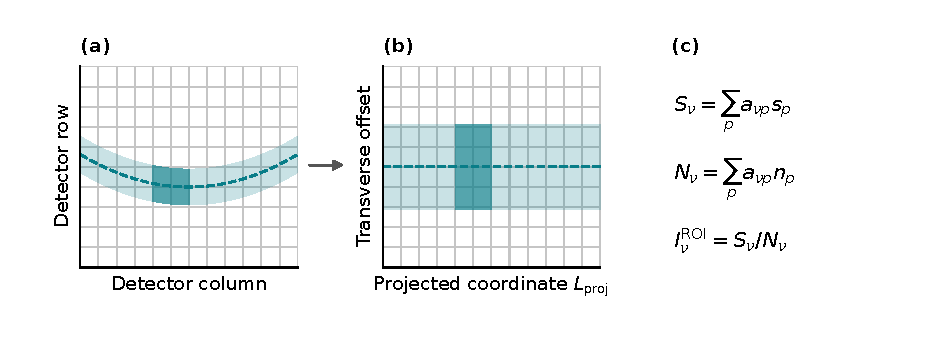
\includegraphics[width=\linewidth]{figures/profile_construction_guide.pdf}
\caption{Construction of a finite-region detector profile. (a) A curved integration band crosses native detector pixels. Teal shading marks accepted area, and the darker segment marks one selected profile interval. (b) A coordinate transformation straightens the band into a strip, where the same darker interval is retained. Gray grid lines show pixel or bin boundaries, and the dashed line marks the trajectory center. (c) Detector signal and normalization pass through the same overlap and mask weights before their accumulated values are divided. The equations define an average over the accepted area.}
\label{fig:si_profile_construction}
\end{figure}

Coordinate and intensity uncertainty are derived in Sec.~\ref{subsec:si_uncertainty}. The finite integration in Fig.~\ref{fig:si_profile_construction} is common to the ordered comparisons in Sec.~\ref{sec:si_ordered_comparisons} and the selected PbI$_2$ profiles in Sec.~\ref{sec:si_pbi2_transition}.

\section{Refraction, absorption, and reflectivity}
\label{sec:si_optics}

The main-text reflectivity discussion separates the low-angle optical response from finite-stack diffraction. The equations below specify the propagation factors and the practical crossover used in the physical diagnostic.

\subsection{Wave propagation, refraction, and absorption}
\label{subsec:si_refraction_absorption}

Let $\zeta\geq0$ denote normal depth into the film and use the field convention
$\exp[i(\widetilde{\mathbf k}\cdot\mathbf r-\omega_{\mathrm{em}}t_{\mathrm{time}})]$. For wavelength sample
$\lambda_s$ with source weight $w_s$,
\begin{equation}
  k_s=\frac{2\pi}{\lambda_s},
  \qquad
  \tilde n_q(\lambda_s)=1-\delta_q(\lambda_s)+i\beta_q(\lambda_s),
  \label{eq:si_complex_n_lambda}
\end{equation}
Here $\widetilde{\mathbf k}$ is the complex optical wavevector, $\mathbf r$ is position and $\tilde n_q$ is the complex refractive index. The prime on an optical wavevector identifies propagation inside the film, as in the main text. The index $s$ is the source-state index, $q$ identifies the optical layer, $\omega_{\mathrm{em}}$ is angular frequency, and $t_{\mathrm{time}}$ is time. The real internal phase vectors used in the main text and Sec.~\ref{sec:si_detector_profiles} are $\mathbf k'_{i,s}=\operatorname{Re}\widetilde{\mathbf k}'_{i,s}$ and $\mathbf k'_{f,s}=\operatorname{Re}\widetilde{\mathbf k}'_{f,s}$. The symbol $\widetilde k_\perp$ below denotes the complex component along the local inward normal. The laboratory $z$ axis is defined separately in Sec.~\ref{sec:si_geometric_ray_acceptance}. The decrement $\delta_q$ controls refraction
and critical-angle behavior, whereas $\beta_q$ controls absorption and
penetration depth. Both are wavelength-dependent material inputs. Their
source, interpolation, and association with the sampled spectrum are recorded
with the calculation configuration.

\paragraph{Tangential matching and the complex normal component.}
Translational invariance along a flat interface conserves the tangential
wavevector. For a field entering layer $q$ from the ambient medium (index $0$), let $\mathbf k_{\parallel,q}$ denote the conserved tangential component. The superscript $(+)$ selects the inward, decaying normal root:
\begin{equation}
  \mathbf k_{\parallel,q}(\lambda_s)
  =\mathbf k_{\parallel,0}(\lambda_s),
  \qquad
  \widetilde k_{\perp,q}^{(+)}(\lambda_s)
  =
  \sqrt{
  \left[\tilde n_q(\lambda_s)k_s\right]^2
  -\left|\mathbf k_{\parallel,0}(\lambda_s)\right|^2}.
  \label{eq:si_boundary_ktz_lambda}
\end{equation}
The root is chosen so that the field decays in its propagation direction. For
the inward solution and the depth convention above,
$\operatorname{Im}\widetilde k_{\perp,q}^{(+)}\geq0$.\cite{Renaud2009} The reciprocal exit
field is obtained from the same boundary condition with its own conserved
tangential component and propagation direction. Real transmitted angles may be reported after this complex-vector calculation. Their evaluation retains both the real and imaginary parts of $\tilde n_q$.

\paragraph{Interface amplitudes and normal flux.}
For a scalar field at an interface from medium $p$ to medium $q$, the field
transmission amplitude is
\begin{equation}
  t_{pq}=\frac{2\widetilde k_{\perp,p}}{\widetilde k_{\perp,p}+\widetilde k_{\perp,q}}.
  \label{eq:si_scalar_transmission}
\end{equation}
Equation~\eqref{eq:si_scalar_transmission} specifies the field-amplitude coefficient. Converting it to a transmitted-flux fraction requires the appropriate flux normalization. In the nonabsorbing scalar limit, the associated
normal-flux ratio includes the factor
$\operatorname{Re}\widetilde k_{\perp,q}/\operatorname{Re}\widetilde k_{\perp,p}$ in addition to
$|t_{pq}|^2$. Absorbing or polarization-resolved layers require the
corresponding Poynting-flux or Fresnel normalization. The calculation must
therefore declare whether each interface weight is a field amplitude, an
intensity, or a normal flux. The transmitted-flux fraction combines $|t_{pq}|^2$ with that normalization.

\paragraph{Normal-depth attenuation.}
Let $\kappa_i(\lambda_s)$ and $\kappa_f(\lambda_s)$ be the nonnegative
imaginary normal components for propagation from the surface to a scattering
depth and from that depth back to the surface, respectively:
\begin{equation}
  \kappa_i(\lambda_s)=\operatorname{Im}\widetilde k_{\perp,i}^{(+)}(\lambda_s),
  \qquad
  \kappa_f(\lambda_s)=\operatorname{Im}\widetilde k_{\perp,f}^{(+)}(\lambda_s),
  \qquad
  \kappa_i,\kappa_f\geq0.
  \label{eq:si_kappa_if_lambda}
\end{equation}
Here \(\widetilde k_{\perp,f}^{(+)}\) is the inward reciprocal exit-channel root used by
reciprocity. Thus \(\kappa_f\) is the positive attenuation constant for the
physical path from depth back to the surface. Equivalently,
\(\kappa_f=-\operatorname{Im}\widetilde k_{\perp,f}^{(\mathrm{out})}\) if an outward
wavevector is stored explicitly.
For a normalized scattering-depth distribution $\rho_{\mathrm{depth}}(\zeta)$ over a film of
thickness $t$, the propagation weight is
\begin{equation}
  W_{\mathrm{depth}}(\lambda_s)=
  \int_0^t \rho_{\mathrm{depth}}(\zeta)
  \exp\!\left[-2\left(\kappa_i(\lambda_s)+\kappa_f(\lambda_s)\right)\zeta\right]d\zeta,
  \qquad
  \int_0^t\rho_{\mathrm{depth}}(\zeta)\,d\zeta=1.
  \label{eq:si_depth_weight_general}
\end{equation}
For uniform scattering density, this becomes
\begin{align}
  W_{\mathrm{depth}}(\lambda_s)
  &=
  \frac{1}{t}\int_0^t
  \exp\!\left[-2\left(\kappa_i(\lambda_s)+\kappa_f(\lambda_s)\right)\zeta\right] d\zeta\\
  &=
  \frac{
  1-\exp\!\left[-2\left(\kappa_i(\lambda_s)+\kappa_f(\lambda_s)\right)t\right]
  }
  {2\left(\kappa_i(\lambda_s)+\kappa_f(\lambda_s)\right)t}.
  \label{eq:si_abs_complex_kz}
\end{align}
Equations~\eqref{eq:si_depth_weight_general} and
\eqref{eq:si_abs_complex_kz} use normal depth. Multiplying
$\operatorname{Im}\widetilde k_\perp$ by an oblique ray-path length would count the angular
projection a second time. The depth weight is combined with consistently
normalized entrance and exit interface factors before it multiplies the
structure-factor and mosaic weights.

\paragraph{Detector accumulation over the bandwidth.}
For each accepted source-state and rod contribution, the wavelength-resolved detector density is formed with
the same geometry, structure-factor, mosaic, detector, and optical interfaces.
The detector images are then added incoherently,
\begin{equation}
  I_{\mathrm{det}}(c_D,r_D)
  =
  \sum_s
  w_s\,
  I_{\mathrm{det},s}\!\left[c_D,r_D;\lambda_s,\{\tilde n_q(\lambda_s)\}\right].
  \label{eq:si_detector_bandwidth_sum}
\end{equation}
Changing $\lambda_s$ changes the moving Ewald construction, the layer optical
constants, the complex normal components, and the interface and depth weights.
The planar-interface correction is retained for every wavelength state. Its
role is expected to be strongest when an incident or exit angle approaches the
critical-angle regime. This optical treatment supplies a propagation correction. Assessing experimental intensity agreement requires measured/calculated comparisons.


\subsection{Parratt-to-kinematic crossover for the axial profile}
\label{subsec:si_parratt_structure_crossover}

The detector-derived $r=0$ profile spans two limiting regimes. The low-$Q_{\mathrm{loc}}$ response is described by standard Parratt reflectivity, while the higher-$Q_{\mathrm{loc}}$ Bragg response is described by a finite-stack kinematic term. The two branches are matched smoothly over a declared overlap interval. We refer to this matching as the Parratt-to-kinematic crossover. It is a practical connection between two established limiting calculations. The main-text reflectivity figure shows measured Bi$_2$Se$_3$ intensities versus detector $2\theta$.

For the physical crossover diagnostic, the dimensionless coordinate is
\begin{equation}
  x=\frac{Q_{\mathrm{loc}}}{Q_c},
  \qquad
  L_{\mathrm{loc}}=\frac{Q_{\mathrm{loc}} c}{2\pi}=x\frac{Q_c c}{2\pi}.
  \label{eq:si_crossover_x_l}
\end{equation}
Here $Q_c$ is the film critical momentum transfer for total external reflection at wavelength $\lambda_s$, and $c$ is the out-of-plane lattice
constant. The transfer $Q_{\mathrm{loc}}=|\mathbf k_{f,s}-\mathbf k_{i,s}|$ is the local momentum-transfer magnitude for specular reflection from a crystallite, whose normal is parallel to that transfer. It generally differs from its mean-film projection $Q_z$. At nominal incidence $\theta_i$, the mean-film specular direction is $2\theta=2\theta_i$. Tilted crystallites can contribute axial scattering away from that direction. The $L_{\mathrm{loc}}$ value in Eq.~\eqref{eq:si_crossover_x_l} is an external local optical coordinate. Finite-stack scattering uses the separate intrinsic phase coordinate. The diagnostic crossover coordinate uses $Q_{\mathrm{loc}}/Q_c$ and the
corresponding $L_{\mathrm{loc}}$ value defined above.

The low-$Q_{\mathrm{loc}}$ branch is the Parratt reflectivity.\cite{Parratt1954} For a layer
$q$ with complex refractive index $\tilde n_q=1-\delta_q+i\beta_q$, the conserved
in-plane wavevector fixes the layer-normal component
\begin{equation}
  \widetilde k_{\perp,q}=\sqrt{(\tilde n_q k_s)^2-\left|\mathbf k_{\parallel}\right|^2},
  \qquad
  k_s=\frac{2\pi}{\lambda_s}.
  \label{eq:si_parratt_kz}
\end{equation}
The fixed source-state label $s$ is suppressed on the layer amplitudes below. For the depth and field convention used above, the square-root branch is chosen
to give decay in the relevant propagation direction.
The superscript $(0)$ labels the smooth-interface coefficient. The Fresnel amplitude at the interface between layers $q$ and $q+1$ is
\begin{equation}
  r_q^{(0)}=\frac{\widetilde k_{\perp,q}-\widetilde k_{\perp,q+1}}{\widetilde k_{\perp,q}+\widetilde k_{\perp,q+1}}.
  \label{eq:si_parratt_interface}
\end{equation}
If the lower interface has RMS roughness $\sigma_{\mathrm{rough},q}$, this coefficient is damped
by
\begin{equation}
  r_q=r_q^{(0)}\exp\!\left[-2\widetilde k_{\perp,q}\widetilde k_{\perp,q+1}\sigma_{\mathrm{rough},q}^2\right].
  \label{eq:si_parratt_roughness}
\end{equation}
For a finite layer of thickness $d_{q+1}$ below the interface, the round-trip
phase factor $P_{\mathrm{opt},q+1}$ is
\begin{equation}
  P_{\mathrm{opt},q+1}=\exp\!\left(2i\widetilde k_{\perp,q+1}d_{q+1}\right).
  \label{eq:si_parratt_phase}
\end{equation}
Starting from the semi-infinite substrate and recursing upward, the effective
reflection amplitude $R_q^{\mathrm{amp}}$ at interface $q$ is
\begin{equation}
  R_q^{\mathrm{amp}}
  =
  \frac{r_q+R_{q+1}^{\mathrm{amp}}P_{\mathrm{opt},q+1}}
       {1+r_qR_{q+1}^{\mathrm{amp}}P_{\mathrm{opt},q+1}}.
  \label{eq:si_parratt_recursion}
\end{equation}
The optical branch in this diagnostic is
\begin{equation}
  R_{\mathrm P}(Q_{\mathrm{loc}})=\left|R_0^{\mathrm{amp}}(Q_{\mathrm{loc}})\right|^2.
  \label{eq:si_parratt_reflectivity}
\end{equation}
This branch retains total external reflection, refraction, evanescence, finite
penetration depth, roughness damping, and multiple reflection between the film
interfaces.

The high-$Q_{\mathrm{loc}}$ branch is built from the normalized finite-stack kinematic term
\begin{equation}
  \widehat S_{00}(L)=
  \frac{S_{q,00}(|\mathbf c^*|L)}{S_{q,00}(0)}.
  \label{eq:si_ht_normalized_structure}
\end{equation}
The hat denotes normalization to the zero-transfer strength, so $\widehat S_{00}(0)=1$. The fixed wavelength $\lambda_s$ is suppressed in these axial structure terms. Here $S_{q,00}$ is the ordered axial structural strength per dimensional rod coordinate from Sec.~\ref{subsec:si_rod_measure}. Near the critical edge, the structure term uses the internal film phase. To match the Parratt film phase, the finite-stack coordinate is computed from the real propagating part of the film wavevector,
\begin{equation}
  Q_{\mathrm{film}}=\operatorname{Re}\!\left(2\widetilde k_{\perp,\mathrm{film}}\right),
  \qquad
  L_{\mathrm{film}}=\frac{Q_{\mathrm{film}}c}{2\pi}.
  \label{eq:si_internal_phase_coordinate}
\end{equation}
Below the critical edge this real part may approach zero in the weak-absorption
limit, while a complex internal wavevector still describes evanescence and
absorption. The superscript $(0)$ on the kinematic branch below labels its unscaled value:
\begin{equation}
  R_{\mathrm{kin}}^{(0)}(Q_{\mathrm{loc}})=\frac{\widehat S_{00}(L_{\mathrm{film}})}{Q_{\mathrm{loc}}^2}.
  \label{eq:si_crossover_unscaled_structure}
\end{equation}
Since $\widehat S_{00}$ is dimensionless, $R_{\mathrm{kin}}^{(0)}$ has units of length squared. It is an unscaled intensity shape. The $Q_{\mathrm{loc}}^{-2}$ factor gives the high-$Q_{\mathrm{loc}}$ structural envelope, while the
internal coordinate $L_{\mathrm{film}}$ keeps the finite-stack fringe phase consistent with
the optical film phase.

A multiplicative scale places this kinematic branch on the Parratt intensity
scale. The scale is fit in a high-$Q_{\mathrm{loc}}$ overlap window, excluding the selected
$00L$ neighborhoods used in the diagnostic. With fit-point index $i$ and retained fit set $\mathcal F$, the
log-median estimate is
\begin{equation}
  A_{\mathrm{opt}}=Q_c^2
  \exp\!\left[
  \operatorname{median}_{i\in\mathcal F}
  \ln\!\left(
  \frac{R_{\mathrm P}(Q_{\mathrm{loc},i})}
       {Q_c^2R_{\mathrm{kin}}^{(0)}(Q_{\mathrm{loc},i})}
  \right)
  \right],
  \label{eq:si_crossover_scale}
\end{equation}
with the default overlap window $5<Q_{\mathrm{loc}}/Q_c<10$. The factors of $Q_c^2$ make the logarithm's argument dimensionless and give $A_{\mathrm{opt}}$ units of inverse length squared. The scaled kinematic branch is therefore dimensionless, like $R_{\mathrm P}$:
\begin{equation}
  R_{\mathrm{kin}}(Q_{\mathrm{loc}})=A_{\mathrm{opt}} R_{\mathrm{kin}}^{(0)}(Q_{\mathrm{loc}}).
  \label{eq:si_crossover_scaled_structure}
\end{equation}

The crossover window is selected by comparing the two positive finite branches in
log intensity. Both branches are evaluated at the same dimensional transfer $Q_{\mathrm{loc}}=Q_c x$:
\begin{equation}
  \delta_{\log}(x)=\log_{10}\!\left[\frac{R_{\mathrm{kin}}(Q_c x)}{R_{\mathrm P}(Q_c x)}\right].
  \label{eq:si_crossover_log_ratio}
\end{equation}
Candidate points must lie in the search range $3\le x\le10$ and satisfy
$|\delta_{\log}(x)|\le0.10$. The selected window $[x_1,x_2]$ is the widest contiguous
eligible region with width at least $1.0$ in $Q_{\mathrm{loc}}/Q_c$. Ties are broken by the
smaller median $|\delta_{\log}|$. If the search rejects every candidate region, the fallback window
is $x_1=3$ and $x_2=6$.

Inside the selected window, the interpolation coordinate and weight are
\begin{equation}
  \eta_{\mathrm{blend}}=\frac{x-x_1}{x_2-x_1},
  \qquad
  w_{\mathrm{blend}}(\eta_{\mathrm{blend}})=6\eta_{\mathrm{blend}}^5-15\eta_{\mathrm{blend}}^4+10\eta_{\mathrm{blend}}^3,
  \label{eq:si_crossover_smoothstep}
\end{equation}
with $\eta_{\mathrm{blend}}$ clipped to the interval $[0,1]$. The final branch is blended in log
reflectivity,
\begin{equation}
R_{\mathrm{blend}}(x)=
\begin{cases}
R_{\mathrm P}(Q_c x), & x\le x_1,\\[3pt]
10^{(1-w_{\mathrm{blend}})\log_{10}R_{\mathrm P}(Q_c x)+w_{\mathrm{blend}}\log_{10}R_{\mathrm{kin}}(Q_c x)},
  & x_1<x<x_2,\\[3pt]
R_{\mathrm{kin}}(Q_c x), & x\ge x_2.
\end{cases}
\label{eq:si_crossover_blend}
\end{equation}
A small positive numerical floor is used only to avoid logarithms of nonpositive
roundoff values inside the blend window. The resulting dimensionless reflectivity is exactly
Parratt below the selected window, exactly the scaled structure branch above the
window, and smooth through the crossover.


The subscript $\mathrm{stitch}$ labels the replacement axial strength after this crossover. The dimensionless blend is converted to the axial structural strength before detector weighting. In the per-$dq_z$ convention of the optical calculation,
\begin{equation}
S_{q,\mathrm{stitch}}(Q_{\mathrm{loc}})
=\frac{Q_{\mathrm{loc}}^2 S_{q,00}(0)}{A_{\mathrm{opt}}}R_{\mathrm{blend}}(Q_{\mathrm{loc}}/Q_c).
\label{eq:si_reflectivity_strength_conversion}
\end{equation}
Above the crossover this recovers the finite-stack strength evaluated at $L_{\mathrm{film}}$. The stitch supplies the replacement axial structural strength and enters the detector weighting once. Equation~\eqref{eq:si_rod_measure_conversion} supplies the conversion to the per-$dL$ density used in Sec.~\ref{sec:si_detector_profiles}.

For the joint comparison, the low-$Q_{\mathrm{loc}}$ interval and the $003$ neighborhood share one normalization. The measured detector profile, the Parratt
branch, the finite-stack branch, and the combined curve must share one declared
background treatment and one intensity scale. The $003$ peak serves as the
higher-$Q_{\mathrm{loc}}$ structural reference. Its sensitivity to wavelength spread can be examined
with Eqs.~\eqref{eq:si_full_spectrum_control} and
\eqref{eq:si_mean_wavelength_control}. The model controls described above
retain the radial extension for a monochromatic source. The contribution of wavelength broadening to the measured feature remains to be established.
Figure~\ref{fig:si_optical_comparison} reserves the physical comparison on that common scale.


\begin{figure}[!htbp]
  \centering
  \siplaceholder{Physical axial reflectivity comparison}{Measured axial profile, direct Parratt and finite-stack branches, combined prediction, and residual.\\Common coordinate map, background, and intensity scale.}
  \caption{Placeholder for the physical axial comparison. The low-angle interval and diffraction region are to be calculated from one declared structural and optical state with uncertainty analysis.}
  \label{fig:si_optical_comparison}
\end{figure}

\section{Additional ordered-film comparisons}
\label{sec:si_ordered_comparisons}

The main text displays the nominal $5^\circ$ Bi$_2$Se$_3$ and Bi$_2$Te$_3$ conditions. This section reserves the direct measured/calculated comparisons needed to assess the ordered-film model. Images at $5^\circ$, $10^\circ$, and $15^\circ$ entered the staged refinement, so comparisons at those conditions assess agreement with the fitted observations.

For each material, the comparison record identifies the exposure, structural input, source distribution, mosaic state, optical assumptions, background, intensity scale, and finite integration regions. Measured and calculated profiles use the same coordinate map and normalization from Sec.~\ref{sec:si_detector_profiles}. A residual is defined as measured minus calculated intensity. Error bars describe the propagated measurement uncertainty and are distinct from numerical convergence errors and parameter uncertainty.

Both detector sides of each retained off-axis family are kept identifiable. Off-axis profiles use $L_{\mathrm{proj}}$, while an axial profile may retain detector $2\theta$ when that is the measured coordinate. A complete comparison preserves negative background-subtracted measurements and records any excluded interval. Figures~\ref{fig:si_bi2se3_profiles} and~\ref{fig:si_bi2te3_profiles} identify the corresponding comparisons.

\begin{figure}[!htbp]
  \centering
  \siplaceholder{Bi$_2$Se$_3$ direct comparisons}{Measured and calculated detector regions.\\Off-axis families on both detector sides and complete axial response.\\Additional incidence angles, residuals, and uncertainties.}
  \caption{Placeholder for Bi$_2$Se$_3$ direct measured/calculated comparisons at the declared incident conditions. Each profile must identify its source state, integration region, normalization, uncertainty, and residual.}
  \label{fig:si_bi2se3_profiles}
\end{figure}


\begin{figure}[!htbp]
  \centering
  \siplaceholder{Bi$_2$Te$_3$ direct comparisons}{Measured and calculated detector regions.\\Off-axis families on both detector sides and complete axial response.\\Additional incidence angles, residuals, and uncertainties.}
  \caption{Placeholder for Bi$_2$Te$_3$ direct measured/calculated comparisons at the declared incident conditions. Each profile must identify its source state, integration region, normalization, uncertainty, and residual.}
  \label{fig:si_bi2te3_profiles}
\end{figure}

\section{PbI\texorpdfstring{$_2$}{2} stacking-disorder model}
\label{sec:si_pbi2_transition}

This section gives the PbI$_2$-specific state construction and the finite-stack
intensity used in the main text.  The general strategy--propagating layer-pair
probabilities with a transition matrix--follows the established theory of
one-dimensionally disordered crystals.\cite{HendricksTeller1942,KakinokiKomura1954,KakinokiKomura1965,Hart2018}
The particular six states, allowed interface events, and fault templates below
are the model assumptions introduced for the present PbI$_2$ analysis.

\subsection{Trilayer amplitudes and six-state basis}

As in the main text, $\rho\in\{0,1,2\}$ labels the basal registry and $\sigma\in\{+,-\}$ labels trilayer orientation. Here $\sigma$ is a discrete state label; the mosaic width $\sigma$ in Sec.~\ref{sec:si_mosaic} is a separate, continuous parameter. The basal registries are
\begin{equation}
  0=(0,0),\qquad
  1=\left(\frac13,\frac23\right),\qquad
  2=\left(\frac23,\frac13\right).
  \label{eq:si_pbi2_registries}
\end{equation}
Taking the Pb plane as the local origin and writing the Pb--I vertical offset
as $\eta=\Delta z_{\mathrm{I-Pb}}/c$, the two orientation-dependent trilayer
amplitudes are
\begin{align}
 F_+(h,k,L)={}&f_{\mathrm{Pb}}+
 f_{\mathrm I}\exp\!\left\{2\pi i\left[\frac{2h+k}{3}+L\eta\right]\right\}
 +f_{\mathrm I}\exp\!\left\{2\pi i\left[\frac{h+2k}{3}-L\eta\right]\right\},
 \label{eq:si_pbi2_Fplus}\\
 F_-(h,k,L)={}&f_{\mathrm{Pb}}+
 f_{\mathrm I}\exp\!\left\{2\pi i\left[\frac{2h+k}{3}-L\eta\right]\right\}
 +f_{\mathrm I}\exp\!\left\{2\pi i\left[\frac{h+2k}{3}+L\eta\right]\right\}.
 \label{eq:si_pbi2_Fminus}
\end{align}
Atomic form factors retain their dependence on $Q=|\mathbf G_{hk}(L)|$ and source wavelength $\lambda_s$. These arguments are suppressed in the matrix expressions below.  The two amplitudes
satisfy $F_-(h,k,L)=F_+(h,k,-L)$.

For the forward registry step $\mathbf{s}=(1/3,2/3)$, define
\begin{equation}
  \omega_{hk}=\exp\!\left[2\pi i(hs_x+ks_y)\right]
  =\exp\!\left[\frac{2\pi i}{3}(h+2k)\right].
  \label{eq:si_pbi2_omega}
\end{equation}
The ordered state basis and its scattering-amplitude vector are
\begin{equation}
 \mathcal{S}=[0F_+,1F_+,2F_+,0F_-,1F_-,2F_-],\qquad
 \mathbf{g}=\begin{pmatrix}
 F_+&\omega_{hk} F_+&\omega_{hk}^2F_+&F_-&\omega_{hk} F_-&\omega_{hk}^2F_-
 \end{pmatrix}^{\mathsf T}.
 \label{eq:si_pbi2_state_amplitudes}
\end{equation}
Because $\omega_{hk}^3=1$, registry 2 is also one backward step from registry 0.

\subsection{Direction-resolved interface law}

The five mutually exclusive interface events are
\begin{equation}
 \boldsymbol{\theta}=(a,b_+,b_-,d_+,d_-),\qquad
 a+b_++b_-+d_++d_-=1.
 \label{eq:si_pbi2_interface_law}
\end{equation}
The entries of $\boldsymbol{\theta}$ are event probabilities. Here $a$ is the probability of retaining both registry and orientation; the basal lattice constant denoted by $a$ in Sec.~\ref{sec:si_structure_factor_conventions} is a different quantity. The $a$ event preserves registry and orientation. The $b_+$ and $b_-$ events shift the
registry by $+1$ and $-1$ while preserving orientation. The $d_+$ and $d_-$ events
combine an orientation change with the two handed shift rules.  Every allowed orientation flip includes a registry shift.  For a $d_+$ event, an $F_+\rightarrow F_-$ step
advances the registry and the corresponding $F_-\rightarrow F_+$ step returns
it.  The directions are interchanged for $d_-$.  This reversal is what makes a
pure $d_+$ or $d_-$ process a deterministic two-layer 4H repeat.

Let
\begin{equation}
 S_+=\begin{pmatrix}0&1&0\\0&0&1\\1&0&0\end{pmatrix},\qquad
 S_-=S_+^{-1}=S_+^{\mathsf T}.
 \label{eq:si_pbi2_shift_matrices}
\end{equation}
The matrices $S_+$ and $S_-$ shift the registry forward and backward, respectively. Let $I_m$ denote the $m$-dimensional identity matrix. With rows denoting the current state and columns the next state, define
\begin{align}
 A&=aI_3+b_+S_+ +b_-S_-,\\
 B&=d_+S_+ +d_-S_-,\\
 C&=d_+S_- +d_-S_+.
\end{align}
Here $A$ is the orientation-preserving block, and $B$ and $C$ are the two orientation-changing blocks. The full six-state transition matrix is
\begin{equation}
 T_6=\begin{pmatrix}A&B\\C&A\end{pmatrix}.
 \label{eq:si_pbi2_T6}
\end{equation}
For example, the row for the state $0F_+$ is
$(a,b_+,b_-,0,d_+,d_-)$.  Every row of $T_6$ sums to one.

The deterministic parent-event vectors, in the order
$(a,b_+,b_-,d_+,d_-)$, are
\begin{equation}
 \mathbf e_{2H}=(1,0,0,0,0),\qquad
 \mathbf e_{4H}=(0,0,0,1,0),\qquad
 \mathbf e_{6H}=(0,1,0,0,0).
 \label{eq:si_pbi2_parent_vectors}
\end{equation}
The opposite-handed 4H and 6H parents are obtained by selecting $d_-$ and
$b_-$ instead.

\subsection{Exact rod-dependent reduction}

The three registry-shift matrices are diagonal in the discrete Fourier basis.
In the sector selected by the scattering phase $\omega_{hk}$, the $6\times6$
transition reduces exactly to
\begin{equation}
 M(\omega_{hk})=
 \begin{pmatrix}
 a+b_+\omega_{hk}+b_-\omega_{hk}^{-1} & d_+\omega_{hk}+d_-\omega_{hk}^{-1}\\
 d_+\omega_{hk}^{-1}+d_-\omega_{hk} & a+b_+\omega_{hk}+b_-\omega_{hk}^{-1}
 \end{pmatrix}.
 \label{eq:si_pbi2_Momega}
\end{equation}
All registry states are retained. Equation~\eqref{eq:si_pbi2_Momega} is one Fourier
block of Eq.~\eqref{eq:si_pbi2_T6}.  Setting the registry phase to unity gives
the orientation-population matrix
\begin{equation}
 P=M(1)=
 \begin{pmatrix}
 a+b_++b_- & d_++d_-\\
 d_++d_- & a+b_++b_-
 \end{pmatrix}.
 \label{eq:si_pbi2_P}
\end{equation}
The matrix $M(\omega_{hk})$ carries complex scattering phases, while $P$ is a row-stochastic probability matrix.

\subsection{Finite-stack intensity}

Let $d$ be the separation between neighboring trilayer centers and
$\xi=\exp(iq_zd)$ the corresponding vertical phase, with $q_z=2\pi L/c$.  Define
\begin{equation}
 \mathbf f=\begin{pmatrix}F_+\\F_-\end{pmatrix},\qquad
 D_{F^*}=\operatorname{diag}(F_+^*,F_-^*).
 \label{eq:si_pbi2_form_vector}
\end{equation}
If $\boldsymbol{\pi}^{\mathrm{ori}}_0$ is the initial orientation row vector,
then the orientation population at trilayer $n$ is
\begin{equation}
 \boldsymbol{\pi}^{\mathrm{ori}}_n
 =\boldsymbol{\pi}^{\mathrm{ori}}_0P^n.
 \label{eq:si_pbi2_orientation_population}
\end{equation}
The vector $\mathbf f$ collects the two orientation amplitudes, and $D_{F^*}$ is their diagonal complex-conjugate matrix. The superscript $\mathrm{ori}$ labels orientation probabilities; each row vector $\boldsymbol{\pi}^{\mathrm{ori}}_n$ sums to one. For integer layer separation $1\leq\Delta<N$, the phase-weighted correlation between trilayers $n$ and $n+\Delta$ is
\begin{equation}
 K_{n,\Delta}=\boldsymbol{\pi}^{\mathrm{ori}}_n
 D_{F^*}M(\omega_{hk})^\Delta\mathbf f.
 \label{eq:si_pbi2_pair_kernel}
\end{equation}
For one fixed parent-rich population $j\in\{2H,4H,6H\}$, the main-text rod intensity uses the per-trilayer convention $S_{hk}^{(j)}=\langle I_N^{(j)}\rangle/N$, where $I_N^{(j)}$ is the intensity of the complete $N$-trilayer stack before the disorder average. Population labels on $F_\pm$, the matrices, and $K_{n,\Delta}$ are suppressed in this single-population derivation. For a finite stack of $N$ trilayers,
\begin{align}
 S_{hk}^{(j)}(L,\lambda_s)={}&
 \frac{1}{N}\sum_{n=0}^{N-1}
 \boldsymbol{\pi}^{\mathrm{ori}}_n
 \begin{pmatrix}|F_+|^2\\|F_-|^2\end{pmatrix}
 \nonumber\\
 &+\frac{2}{N}\operatorname{Re}\!\left[
 \sum_{\Delta=1}^{N-1}\xi^\Delta
 \sum_{n=0}^{N-1-\Delta}K_{n,\Delta}\right].
 \label{eq:si_pbi2_finite_intensity}
\end{align}
The connection to the main-text pair-correlation notation is
\begin{equation}
 C_{hk}^{(j)}(\Delta;L,\lambda_s)
 =\frac{1}{N-\Delta}\sum_{n=0}^{N-1-\Delta}K_{n,\Delta},
 \qquad 1\leq\Delta<N.
 \label{eq:si_pbi2_main_correlation}
\end{equation}
The first term in Eq.~\eqref{eq:si_pbi2_finite_intensity} is $S_{\mathrm{self},hk}^{(j)}(L,\lambda_s)$. Since $\xi^\Delta=e^{iq_zd\Delta}$, grouping the pair sum with this definition gives the main-text finite-stack expression directly.

The first term contains the $N$ self contributions and the second contains all
distinct trilayer pairs.  The calculation evaluates these finite sums
directly, retaining end effects and avoiding singular closed forms when an
eigenvalue approaches unity.  Equivalent matrix-power and recursive
formulations are standard for planar-fault diffraction.\cite{Treacy1991}

\subsection{Polytype-rich fault templates and population mixture}

For each parent-rich population,
\begin{equation}
 \boldsymbol{\theta}_j(\epsilon_j)
 =(1-\epsilon_j)\mathbf e_j+\epsilon_j\mathbf q_j,
 \qquad j\in\{2H,4H,6H\}.
 \label{eq:si_pbi2_fault_parameterization}
\end{equation}
Here $\mathbf e_j$ is the deterministic parent-event vector, $\mathbf q_j$ is the probability vector for a fault event, and $0\leq\epsilon_j\leq1$ is its probability. The equal-alternative templates used in the present implementation are
\begin{align}
 \mathbf q_{2H}&=\left(0,\frac14,\frac14,\frac14,\frac14\right),\\
 \mathbf q_{4H}&=\left(\frac14,\frac14,\frac14,0,\frac14\right),\\
 \mathbf q_{6H}&=\left(\frac14,0,\frac14,\frac14,\frac14\right).
 \label{eq:si_pbi2_fault_templates}
\end{align}
Consequently, $\epsilon_j$ is exactly the probability that an interface in
population $j$ follows one of the four alternative events. Its numerical value is conditional on the chosen $\mathbf q_j$ and is interpreted together with that template.

The parent-rich populations are mutually incoherent, with nonnegative weights $w_j$ that sum to one. Their structural intensities combine using the main-text notation:
\begin{equation}
 S_{hk}(L,\lambda_s)=\sum_{j\in\{2H,4H,6H\}}
 w_jS_{hk}^{(j)}(L,\lambda_s),\qquad
 w_{2H}+w_{4H}+w_{6H}=1.
 \label{eq:si_pbi2_total_intensity}
\end{equation}
The detector/profile prediction, background, scale and optional finite-profile kernel are specified separately in Sec.~\ref{subsec:si_detector_derived_objectives}.
The core parameterization has three disorder magnitudes and two independent
population weights.  The stack length $N$, scale, and any fixed or refined
finite-profile and instrumental broadening terms are separate.  When three independent disorder magnitudes remain underconstrained, the constrained starting model is
$\epsilon_{2H}=\epsilon_{4H}=\epsilon_{6H}$.

\subsection{Deterministic and phase-insensitive checks}

Table~\ref{tab:si_parent_cycles} gives the zero-disorder cycles.
\begin{table}[!htbp]
\centering\small
\caption{Deterministic PbI$_2$ parent cycles from the initial state $0F_+$. Each row specifies the unit-probability interface event, its registry/orientation cycle, and the corresponding reduced transfer matrix. The phase $\omega_{hk}$ is defined in Eq.~\eqref{eq:si_pbi2_omega}; $I_2$ is the two-dimensional identity matrix.}
\label{tab:si_parent_cycles}
\begin{tabular}{llll}
\toprule
Parent & Nonzero event & State cycle from $0F_+$ & Reduced matrix\\
\midrule
2H & $a=1$ & $0F_+\rightarrow0F_+$ & $I_2$\\
4H & $d_+=1$ & $0F_+\rightarrow1F_-\rightarrow0F_+$ &
$\left(\begin{smallmatrix}0&\omega_{hk}\\\omega_{hk}^{-1}&0\end{smallmatrix}\right)$\\
6H & $b_+=1$ & $0F_+\rightarrow1F_+\rightarrow2F_+\rightarrow0F_+$ &
$\omega_{hk} I_2$\\
\bottomrule
\end{tabular}
\end{table}
\FloatBarrier
For 4H, $M(\omega_{hk})^2=I_2$. For 6H, $M(\omega_{hk})^3=I_2$ because
$\omega_{hk}^3=1$.  The $d_-=1$ and $b_-=1$ limits generate the opposite-handed
cycles.

For $h=k=0$, $\omega_{hk}=1$ and $F_+=F_-=F$.  Because $P^\Delta\mathbf 1=\mathbf 1$, where $\mathbf 1=(1,1)^{\mathsf T}$, Eq.~\eqref{eq:si_pbi2_pair_kernel} becomes
$K_{n,\Delta}=|F|^2$ for every allowed transition law.  Equation
\eqref{eq:si_pbi2_finite_intensity} then reduces to the normalized Laue factor
\begin{equation}
 S_{00}^{(j)}(L,\lambda_s)
 =\frac{|F|^2}{N}\left|\sum_{n=0}^{N-1}\xi^n\right|^2
 =\frac{|F|^2}{N}\frac{\sin^2(N\vartheta/2)}{\sin^2(\vartheta/2)},
 \qquad \vartheta=q_zd,\quad \xi=e^{i\vartheta}.
 \label{eq:si_pbi2_r0_laue}
\end{equation}
Thus the strong $r=0$ oscillations are finite-thickness fringes. The included registry and orientation paths are contrast-matched on this rod, so faults can remain present with the same axial intensity. Figure~\ref{fig:si_pbi2_transition_validation} reserves the direct numerical checks of these limits. Figure~\ref{fig:si_pbi2_sensitivity} separates the effects of faults within a stack from changes in population weights.


\begin{figure}[!htbp]
  \centering
  \siplaceholder{PbI$_2$ model verification}{(a) Full six-state and reduced calculations.\\(b) Deterministic 2H, 4H, and 6H limits.\\(c) Axial invariance across transition laws.}
  \caption{Placeholder for verification of the PbI$_2$ model. Direct arrays will compare the full and reduced expressions, independent deterministic-parent sums, and the phase-insensitive axial limit.}
  \label{fig:si_pbi2_transition_validation}
\end{figure}


\begin{figure}[!htbp]
  \centering
  \siplaceholder{PbI$_2$ disorder and population sensitivity}{(a) One fault probability varied at fixed population weights.\\(b) Population weights varied at fixed transition laws.\\Shared axes and declared structural assumptions.}
  \caption{Placeholder for direct PbI$_2$ sensitivity calculations. Separate controlled panels distinguish within-stack fault probabilities from incoherent population weights.}
  \label{fig:si_pbi2_sensitivity}
\end{figure}

\section{Calibration, refinement, and uncertainty}
\label{sec:si_workflow}

The main-text workflow separates parameter groups because several effects can change the same peak position, width, or intensity. This section defines the stage-specific observables and the propagation of uncertainty through the shared detector integration.

\subsection{Parameter groups and calibration}

\begin{enumerate}
  \item \textbf{Beam characterization (direct beam).}
  Direct-beam spot positions and shapes at several detector distances constrain the incident-beam widths $(w_x,w_z)$ and Gaussian divergences $(\Delta\theta_x,\Delta\theta_z)$ that set the instrument-limited broadening.

  \item \textbf{Detector geometry calibration (3D powder standard).}
  Dark-subtracted Debye--Scherrer rings from a polycrystalline hBN calibrant constrain detector distance, detector tilts $(\beta_D,\gamma_D)$, in-plane detector rotation $\chi_D$, and beam center $(x_0,y_0)$.

  \item \textbf{Sample alignment and goniometer misalignment.}
  Indexed Bragg-peak centers constrain sample alignment with the detector parameters fixed. The positional objective minimizes detector-space residuals between measured and calculated peak positions spanning both specular and off-specular regions. Here $\theta_i$ is grazing incidence, $\chi$ is the in-plane sample rotation, and $z_B$ and $z_S$ are the beam and sample height coordinates in the laboratory frame. The adjustable quantities are $(\theta_i,\chi,z_B,z_S)$ and the goniometer-axis misalignment rotations $(\alpha_{\mathrm{gon}},\psi)$. Here $\alpha_{\mathrm{gon}}$ denotes the alignment angle labeled $\alpha$ in the main-text workflow table; the subscript distinguishes it from the crystallite tilt $\alpha$ in Sec.~\ref{sec:si_mosaic}. Finite film dimensions $(W,H)$ enter only when finite support is selected, while thickness $t$ enters the absorption model. The retained ordered-film geometry uses the unbounded in-plane support described in Sec.~\ref{sec:si_geometric_ray_acceptance}.

  \Needspace{4\baselineskip}
  \item \textbf{Mosaicity/profile refinement.}
  With geometry fixed, selected local detector regions or local $I(\phi_f)$ profiles after center alignment constrain mosaicity. The shared profile model is a wrapped two-component angular distribution with a Gaussian-like core and a Lorentzian-like broad component. The two components have independent widths. Off-specular arcs mainly inform the narrow core, while off-condition axial intensity is sensitive to the broad component together with bandwidth, divergence, alignment, and background. The parameterization yields component widths and a broad-component weight, but attribution and necessity require the controlled no-tail and re-optimized Gaussian-only comparisons at fixed remaining parameters and after refitting, respectively.

  \item \textbf{Ordered-structure refinement.}
  With geometry and mosaicity fixed, the ordered intensity objective compares the model with background-subtracted integrated counts in selected detector-space Bragg regions of interest (ROIs) from multiple dark-subtracted images. The corresponding prediction integrates the calculated detector density over those same ROIs. The objective permits one nuisance scale per image and physically constrained ordered-structure parameters.

  \item \textbf{Disorder refinement.}
  After the ordered baseline is established, stacking-disorder parameters enter through fixed-in-plane-momentum rod profiles reported versus the film-normal momentum. The measured profile is formed from caked signal and normalization fields by summing signal and normalization over the selected rod mask before division. Geometry, detector calibration, beam terms, mosaicity, lattice constants, and the ordered baseline remain fixed. Only stacking-disorder parameters and declared scale/background terms are refined.
\end{enumerate}

All detector images are dark-subtracted before fitting. Any additional flat-field, polarization, or detector-efficiency correction enters the common intensity convention for the compared images. The calculated detector density already includes the pixel solid-angle factor. Applying that factor again would duplicate the correction. Stage-specific uncertainty could be estimated by repeated constrained refits, resampling calibrant points for detector geometry, indexed peak lists for sample alignment, local reflection regions for mosaicity, accepted Bragg regions for ordered intensity, and selected rod bins for disorder. The spread of the accepted solutions would then quantify uncertainty within each stage and contribute to uncertainty in subsequent stages.

The hBN calibration requires a reproducible record of the selected rings, masks, fitted geometry, positional residuals, and uncertainty. Likewise, a final parameter table must distinguish fixed structural inputs from refined values and link each value to the calculation state used for the comparisons in Sec.~\ref{sec:si_ordered_comparisons}.

\subsection{Ordered-intensity and disorder objectives}
\label{subsec:si_detector_derived_objectives}

The detector-space forward model predicts a continuous detector-coordinate density and its finite-region integrals, while the inverse problems use stage-specific observables. In the ordered-structure stage, the measured quantity for ROI $i$ in exposure $e$ is the background-subtracted detector count
\[
  y_{ei}=\sum_{(c_D,r_D)\in\Omega_{ei}}\left[I_e^{\mathrm{meas}}(c_D,r_D)-b_{ei}(c_D,r_D)\right],
\]
Here $I_e^{\mathrm{meas}}$ is the native pixel count in exposure $e$, $\Omega_{ei}$ is the selected detector-space Bragg ROI and $b_{ei}$ is its local background count model. The sum runs over pixel centers within that ROI. The corresponding prediction is the detector-coordinate density integrated over the same region,
\[
  \mu_{ei}=\int_{\Omega_{ei}} I_{\mathrm{det},e}^{\mathrm{calc}}(c_D,r_D)\,dc_D\,dr_D,
\]
or the equivalent deterministic sum of native pixel masses. Geometry, source terms, and mosaicity are fixed before this stage. One nuisance scale per image accounts for exposure and flux differences. This defines a multi-image ordered-intensity objective restricted to the selected Bragg ROIs.

The PbI$_2$ disorder refinement is restricted to the final-stage selected profiles. The upstream beam, detector, sample alignment, mosaic/profile parameters, lattice constants, and ordered PbI$_2$ baseline are fixed before this stage starts. The measured selected-rod profile is the signal-to-normalization ratio in Eq.~\eqref{eq:si_profile_average}. Its reciprocal-space mask and detector-side selection remain fixed during this stage.

The parameter vector $\boldsymbol{\Theta}_{\mathrm{dis}}$ contains the released fault probabilities and independent population weights, together with $N$ if stack length is refined. The model profile is evaluated along the same selected branch. A scalar convolution approximates the detector response when its variation along that branch can be represented by a fixed kernel. In the common intrinsic-$L$ coordinate used for that approximation,
\begin{equation}
 I_\nu^{\mathrm{calc}}(\boldsymbol{\Theta}_{\mathrm{dis}})
 =B_{\mathrm{bg}}(x_\nu)+a_{\mathrm{sc}}
 \left[K_{\mathrm{prof}}*\sum_{j\in\{2H,4H,6H\}}
 w_jS_{hk}^{(j)}(L,\lambda_s;\epsilon_j,N)\right]_\nu.
 \label{eq:si_disorder_profile_model}
\end{equation}
Here $\nu$ labels a retained profile bin, $x_\nu$ is its displayed coordinate, $B_{\mathrm{bg}}$ is the low-order background, $a_{\mathrm{sc}}$ is a common intensity scale, and $K_{\mathrm{prof}}$ is the fixed finite-profile kernel. The binary $*$ denotes convolution in intrinsic $L$. The bracket denotes evaluation and integration over the same selected bin as the measurement. The source wavelength and other upstream inputs are fixed in this compact single-state expression; a source ensemble is accumulated with the weights $w_s$ before the same profile extraction. The structural functions $S_{hk}^{(j)}$ are those of Sec.~\ref{sec:si_pbi2_transition}. Kernel widths are fixed by the upstream resolution and mosaic state or declared before the fit; peak areas remain governed by the structural model.

The scale and background arguments are suppressed in $I_\nu^{\mathrm{calc}}$; they remain explicit in the objective. The disorder objective uses only the retained profile-bin set $\mathcal V$:
\begin{equation}
 \Phi_{\mathrm{dis}}(\boldsymbol{\Theta}_{\mathrm{dis}},a_{\mathrm{sc}},B_{\mathrm{bg}})
 =\sum_{\nu\in\mathcal V}\mathcal L\!\left(
 \frac{I_\nu^{\mathrm{ROI}}-I_\nu^{\mathrm{calc}}(\boldsymbol{\Theta}_{\mathrm{dis}})}{\sigma_{I,\nu}}
 \right).
 \label{eq:si_disorder_objective}
\end{equation}
Here $I_\nu^{\mathrm{ROI}}$ is the measured ratio defined in Eq.~\eqref{eq:si_profile_average}, $\sigma_{I,\nu}^2=\mathrm{Var}(I_\nu^{\mathrm{ROI}})$ is its intensity variance, and $\mathcal L$ is the declared loss function. For standardized residual $v$, the choice $\mathcal L(v)=v^2$ gives the usual pointwise least-squares objective; a robust loss defines a different objective. Correlated profile bins require the covariance treatment below. The fixed detector geometry and ordered model determine the known Bragg locations. Fitting independent peak amplitudes before the stacking model would absorb the diffuse between-peak intensity into preprocessing.

\subsection{Coordinate and intensity uncertainty}
\label{subsec:si_uncertainty}

The transformed-coordinate uncertainty has two parts: uncertainty in the coordinate label and uncertainty in the rebinned intensity. The coordinate-label uncertainty follows from the finite detector-pixel footprint and from uncertainty in the detector calibration. For square detector pixels with pitch $p_{\mathrm{pix}}$ and reference detector distance $D$, the leading flat-detector terms are
\begin{equation}
\sigma_{2\theta,\mathrm{pix}}(2\theta)=
\frac{p_{\mathrm{pix}}\cos^{2}(2\theta)}{\sqrt{12}\,D},
\qquad
\sigma_{\phi_f,\mathrm{pix}}(2\theta)=
\frac{p_{\mathrm{pix}}}{\sqrt{12}\,D\tan(2\theta)}.
\end{equation}
The radial term is finite and largest near the direct beam. The azimuthal term scales as $1/\tan(2\theta)$, so azimuth is poorly conditioned near the direct-beam direction, where $2\theta$ approaches zero.

For the $D=75$ mm and $p_{\mathrm{pix}}=300\,\mu\mathrm{m}$ geometry used in the uncertainty calculation, the maximum radial coordinate uncertainty is approximately $0.066^{\circ}$. The azimuthal coordinate uncertainty falls below $1^{\circ}$ above $2\theta\approx3.8^{\circ}$, below $0.5^{\circ}$ above $2\theta\approx7.5^{\circ}$, and below $0.25^{\circ}$ above $2\theta\approx14.9^{\circ}$. More generally, the threshold for a target azimuthal width $w_{\phi_f}$ is
\begin{equation}
2\theta_{\mathrm{crit}}=\arctan\!\left(\frac{p_{\mathrm{pix}}}{\sqrt{12}\,D\,w_{\phi_f}}\right),
\end{equation}
with $w_{\phi_f}$ expressed in radians.

Additional calibration uncertainty can be propagated with the usual Jacobian form. If the uncertain geometry parameters are collected in $\mathbf g_{\mathrm{cal}}$ with covariance matrix $\Sigma_{\mathrm{cal}}$, the row Jacobians are $J_{2\theta}=\partial(2\theta)/\partial\mathbf g_{\mathrm{cal}}$ and $J_{\phi_f}=\partial\phi_f/\partial\mathbf g_{\mathrm{cal}}$. The propagated variances are
\begin{equation}
\sigma^2_{2\theta,\mathrm{cal}}=
J_{2\theta}\Sigma_{\mathrm{cal}}J_{2\theta}^{\mathsf T},
\qquad
\sigma^2_{\phi_f,\mathrm{cal}}=
J_{\phi_f}\Sigma_{\mathrm{cal}}J_{\phi_f}^{\mathsf T}.
\end{equation}
If the displayed bin-center label is also treated as uncertain, the bin widths $\Delta(2\theta)$ and $\Delta\phi_f$ contribute
\begin{equation}
\sigma^2_{2\theta,\mathrm{bin}}=\frac{[\Delta(2\theta)]^2}{12},
\qquad
\sigma^2_{\phi_f,\mathrm{bin}}=\frac{(\Delta\phi_f)^2}{12}.
\end{equation}
These coordinate terms describe the uncertainty of the transformed axis value. They are separate from intensity uncertainty.

The intensity uncertainty is inherited from the detector through the same overlap weights used to construct the caked image and the projected profile. If $v_p$ is the detector-pixel variance and the detector-pixel variances are independent, then
\begin{equation}
\mathrm{Var}\!\left(I_{\nu}^{\mathrm{ROI}}\right)=
\frac{\sum_p a_{\nu p}^{2}v_p}
     {\left(\sum_p a_{\nu p}n_p\right)^2}.
\end{equation}
If overlapping interpolation weights are used, neighboring profile points can be statistically correlated. For profile bins $\nu$ and $\nu'$, the corresponding covariance is
\begin{equation}
\mathrm{Cov}\!\left(I_{\nu}^{\mathrm{ROI}},I_{\nu'}^{\mathrm{ROI}}\right)=
\frac{\sum_p a_{\nu p}a_{\nu'p}v_p}
     {\left(\sum_p a_{\nu p}n_p\right)
      \left(\sum_p a_{\nu'p}n_p\right)}.
\end{equation}
Thus the same weights that define the projected profile also propagate the detector-pixel variance. This expression assumes fixed normalization and masks and independent input-pixel variances. Correlated background or calibration errors require additional covariance terms. Off-diagonal covariance terms describe correlations between neighboring projected points.

The displayed coordinate for a projected point can be represented by the same finite-band weighting. For example,
\begin{equation}
\bar L_{\mathrm{proj},\nu}=\frac{\sum_b \mu_{\nu b}N_bL_{\mathrm{proj},b}}{\sum_b \mu_{\nu b}N_b},
\qquad
\sigma^2_{L_{\mathrm{proj}},\nu}=\frac{\sum_b \mu_{\nu b}N_b(L_{\mathrm{proj},b}-\bar L_{\mathrm{proj},\nu})^2}{\sum_b \mu_{\nu b}N_b},
\end{equation}
Here $\bar L_{\mathrm{proj},\nu}$ is the weighted coordinate mean, $\sigma^2_{L_{\mathrm{proj}},\nu}$ is its finite-band variance, and $L_{\mathrm{proj},b}$ is the coordinate at caked bin $b$. These terms precede the addition of calibration, incidence-angle, wavelength, divergence, and mosaic contributions. This width describes the finite-bin projection. Counting-statistical intensity uncertainty is propagated separately through the detector-pixel variances.

These projection uncertainties are coupled to model-parameter correlations. Peak positions are sensitive to detector distance, beam center, detector tilt, sample height, and incidence angle. Profile widths are sensitive to both beam divergence and the Gaussian mosaic core. Off-condition profiles are sensitive to the broad mosaic component together with bandwidth, divergence, alignment, and background. Near-critical intensity additionally depends on the optical response and is excluded from evidence for the broad component. Relative integrated intensities are sensitive to scale, footprint, absorption, thickness, and structure-factor parameters. The staged workflow separates these effects by fixing or constraining the parameters tied to peak position before fitting profile widths, and by fixing the geometry and mosaic state before interpreting ordered intensities.

These expressions give four practical consequences. First, the $2\theta$--$\phi_f$ maps and $Q_R$-selected $Q_z$ profiles are controlled projections that inherit the detector image's finite resolution and statistical information. Second, transformed-coordinate uncertainty is concentrated at low angles near the direct beam. Third, intensity variance is propagated through the same overlap weights used for caking and profile extraction. Fourth, the strongest remaining systematic coupling occurs near low $L$, where direct-beam background, bandwidth, divergence, incidence angle, and optical response overlap. That near-critical region is excluded from evidence for the broad mosaic component.

\subsection{Numerical evaluation and convergence}

The physical sequence is source sampling, sample acceptance, internal propagation, orientation-weighted Ewald selection, exit propagation, detector mapping, and finite-region integration. The forward roots in Sec.~\ref{subsec:si_ewald_surface_chart} and inverse detector evaluation describe the same compatible scattering states. Numerical source sampling integrates the incident-beam distribution, while the separate mosaic law specifies crystallite orientations.

Source-state count and detector integration order control different approximations. A convergence comparison holds the physical parameters, masks, background and count scale fixed while changing one numerical setting at a time. Agreement is assessed for the actual detector regions and profiles used in the manuscript, including narrow peaks and low-angle regions. Establishing convergence requires quantitative agreement under these changes in numerical settings. Figure~\ref{fig:si_convergence} reserves the corresponding numerical comparison.


\begin{figure}[!htbp]
  \centering
  \siplaceholder{Numerical convergence}{(a) Source-state count at fixed integration order.\\(b) Integration order at fixed source ensemble.\\Profile differences and integrated-intensity changes in declared regions.}
  \caption{Placeholder for numerical convergence of the detector observables. The intended comparison reports source sampling and finite-area quadrature separately, with fixed physical inputs and explicit tolerances.}
  \label{fig:si_convergence}
\end{figure}

\FloatBarrier
\clearpage
\bibliographystyle{apsrev4-2}
\bibliography{../bibliography/references}
\end{document}
